\documentclass[a4paper,12pt,oneside]{article}

% Imported packages
\usepackage[english]{babel}
\usepackage[T1]{fontenc}
\usepackage[utf8]{inputenc}
\usepackage{amssymb}
\usepackage{amsmath}
\usepackage{bm}
\usepackage{listings}
\usepackage{graphicx}
\usepackage{geometry}
\usepackage{float}
\usepackage{subfigure}
\usepackage{wrapfig}
\usepackage{comment}
\usepackage{hyperref}

% Margin dimensions settings
\geometry{a4paper,top=2cm,bottom=2cm,left=2cm,right=2cm,
heightrounded,bindingoffset=5mm}

% Enumeration settings
\renewcommand{\thesubsection}{\thesection.\alph{subsection}}

% Reset section counter with new part
%\makeatletter
%\@addtoreset{section}{part}
%\makeatother
%\renewcommand{\thesection}{\Alph{section}}
%\renewcommand{\thesubsection}{\arabic{subsection}}
%\newcommand{\tipologia}[1]{%
%  \stepcounter{part}% Ecco il trucco
%  \section*{Tipologia \thesection. #1}}


% Code visualization settings
\lstset{basicstyle=\small\ttfamily}

% Code design settings
\lstset{language=Matlab}

% Included images path
\graphicspath{{Images/}}

% Document information
\title{Fundamentals of Vibration Analysis and Vibroacoustics \\
Module 1 - Fundamentals of Vibration Analysis \\
Assignment 3 - Modal parameter identification}
\author{Bombaci Nicola 10677942 \\
Fantin Jacopo 10591775 \\
Intagliata Emanuele 10544878}
\date{May 2020}


\begin{document}

\maketitle

\vspace{100pt}

In this problem, we're given a small set of measurements we have to extract information from. The virtual experiment consists in a hammer hitting impulsively a structure in one point, and measuring the displacements in four different positions, one of which is where the force is applied (the first one). The initial data are wherefore the time axis $ t $ used to represent the sampled measurements and the force, the impulse-like input force $ F(t) $, and the four measurements:

\[
	t ~ \text{,} ~ F(t) ~ \text{,} ~
		x_1(t) ~ \text{,} ~ x_2(t) ~ \text{,} ~ x_3(t) ~ \text{,} ~ x_4(t)
\]

\section{Experimental FRFs}
\label{sec:experimental_frfs}

The Frequency Response Functions linking the displacement of the four points to the external force can be retrieved computing the ratio between the Discrete Fourier Transform (DFT) of the former and of the latter. We used the Matlab function \lstinline!fft! to find the DFT of the function input, here denoted with $ \mathcal{F[\cdot]} $, through an optimized Fast Fourier Transform algorithm.

%\begin{lstlisting}
%	H_exp = [fft(x1)./fft(F);
%		 fft(x2)./fft(F);
%		 fft(x3)./fft(F);
%		 fft(x4)./fft(F)];
%\end{lstlisting}

\[
	H^\textup{exp}_k(f) = \frac{\mathcal{F}[x_k(t)]}{\mathcal{F}[F(t)]}
		~ \text{,} ~ k = 1,2,3,4
\]

Note that the first element $ H^\textup{exp}_1(f) $ represents the co-located FRF. The corresponding plots are represented in magnitude and phase as follows:

\begin{figure}[H]
	\hspace{-70pt}
	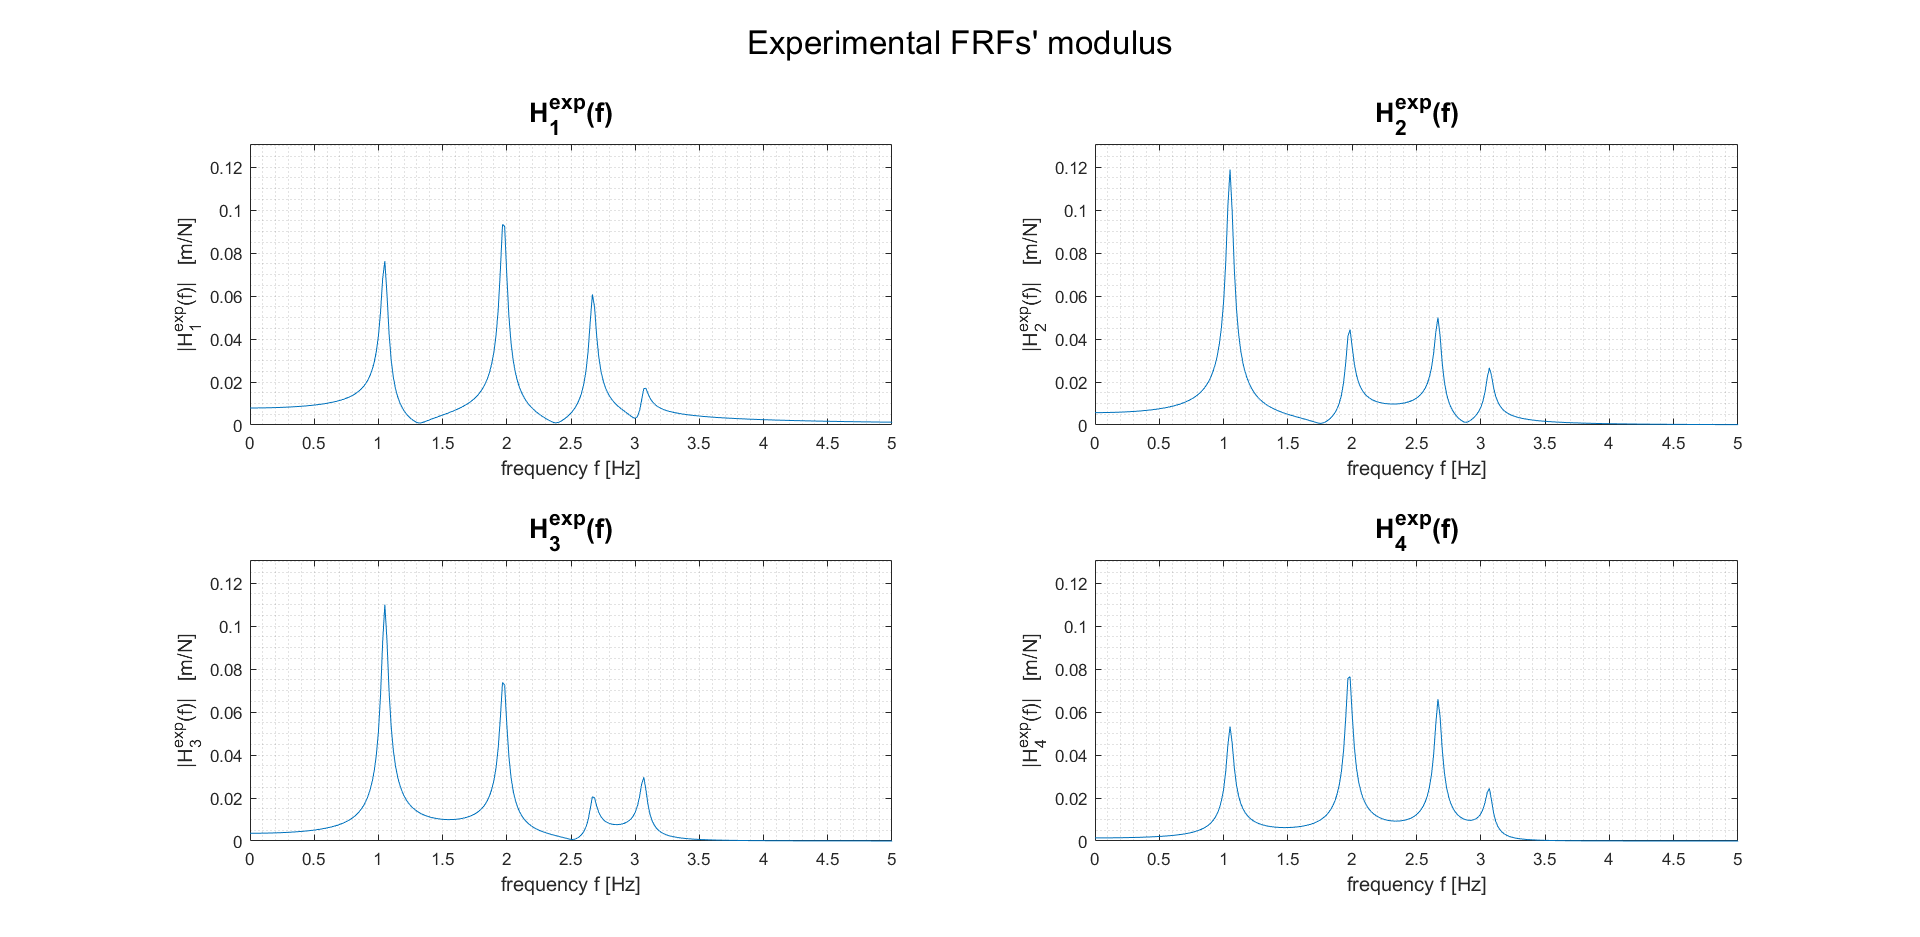
\includegraphics[scale=0.4]{experimental_frfs_modulus}
\end{figure}

\begin{figure}[H]
	\hspace{-70pt}
	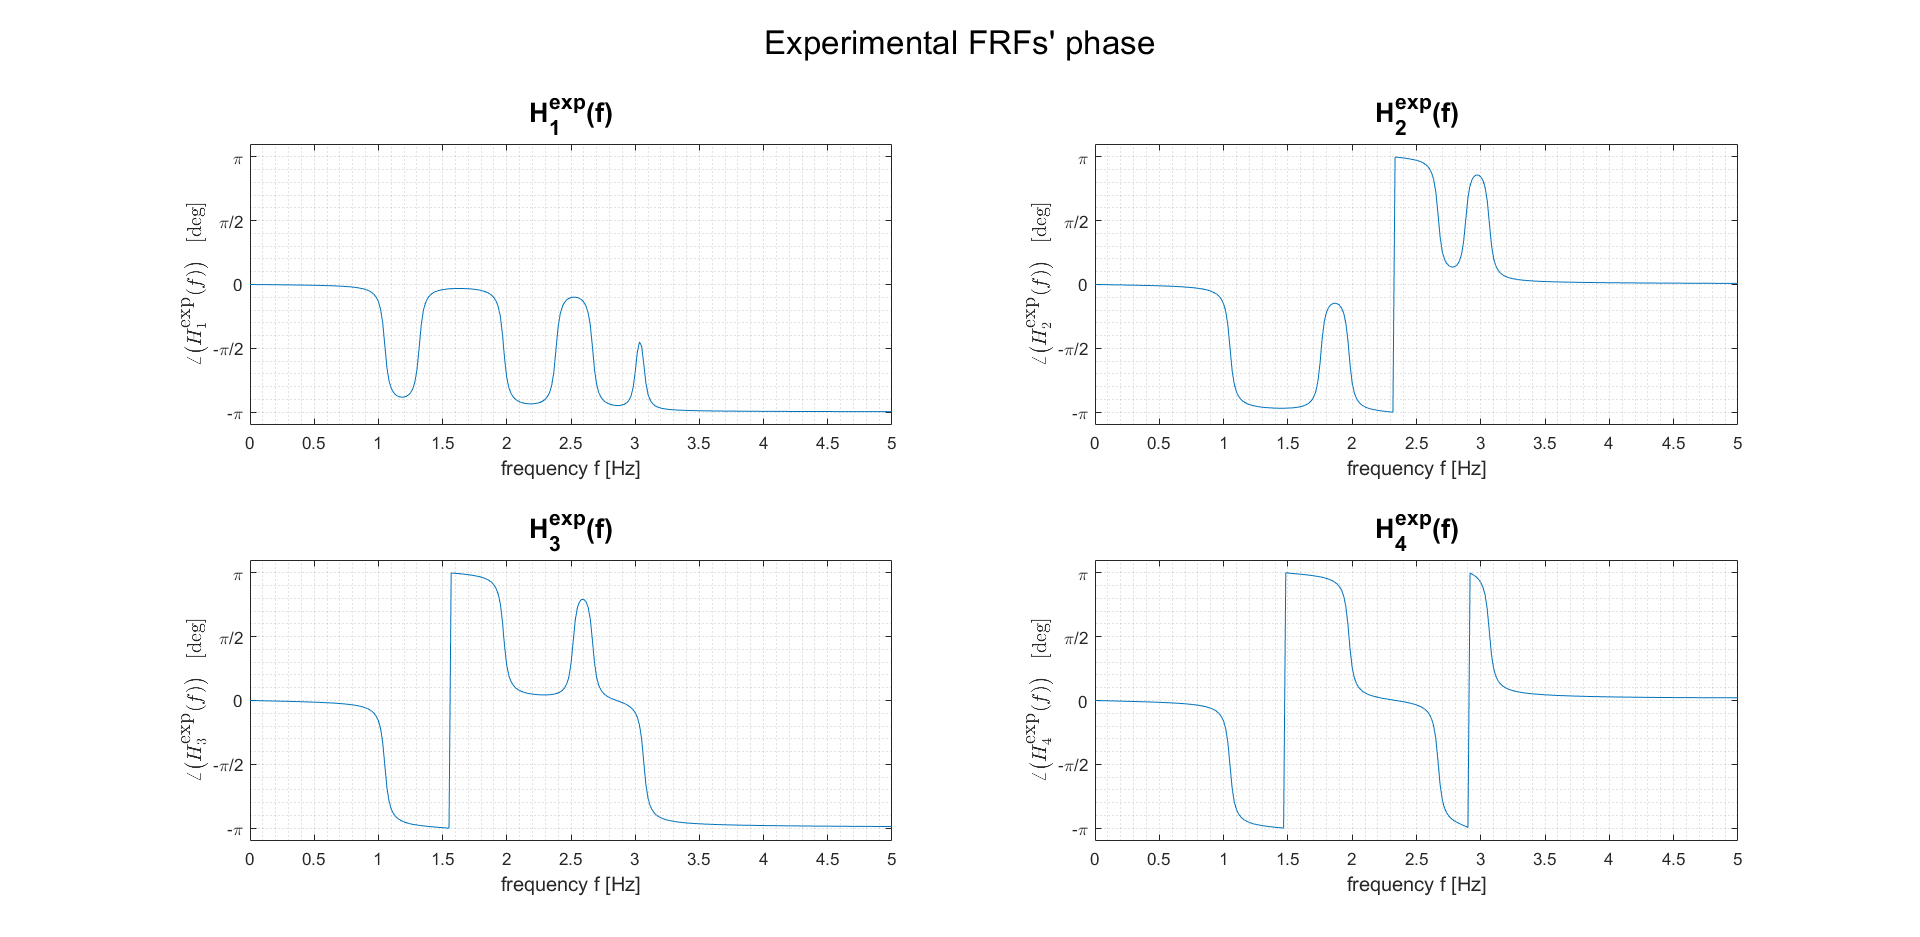
\includegraphics[scale=0.4]{experimental_frfs_phase}
\end{figure}


\section{Simplified methods for model identification}
\label{sec:simplified_methods}

To estimate the system parameters, we first reached for simplified methods. The assumption we are working under are, as usual, low damping (order of magnitude for $ \xi $: $ 10{-2} $), and well-distincted peaks in amplitude spectrum. As long as the damped frequencies are concerned, we found the relative maxima in each FRF setting one order of magnitude lower than the absolute maximum as threshold, and then found the frequencies corresponding to those values. The resulting matrix of damped frequencies is:

\[
	\mathbf{f_d} =	\begin{bmatrix}
										f_{\textup{d}_1}^{(1)}	& f_{\textup{d}_1}^{(2)} &
											f_{\textup{d}_1}^{(3)}	& f_{\textup{d}_1}^{(4)} \\
										f_{\textup{d}_2}^{(1)}	& f_{\textup{d}_2}^{(2)} &
											f_{\textup{d}_2}^{(3)}	& f_{\textup{d}_2}^{(4)} \\
										f_{\textup{d}_3}^{(1)}	& f_{\textup{d}_3}^{(2)} &
											f_{\textup{d}_3}^{(3)}	& f_{\textup{d}_3}^{(4)} \\
										f_{\textup{d}_4}^{(1)}	& f_{\textup{d}_4}^{(2)} &
											f_{\textup{d}_4}^{(3)}	& f_{\textup{d}_4}^{(4)} \\
									\end{bmatrix} = \begin{bmatrix}
																		1.0500	& 1.9667	& 2.6667	& 3.0833 \\
																		1.0500	& 1.9833	& 2.6667	& 3.0667 \\
																		1.0500	& 1.9667	& 2.6667	& 3.0667 \\
																		1.0500	& 1.9833	& 2.6667	& 3.0667
																	\end{bmatrix}
\]

where every row corresponds to one of the four different measurements, and each column to a vibration mode. The values are affected by small fluctuations as for the 2\textsuperscript{nd} and 4\textsuperscript{th} frequency, so we can reckon the values overall agree with each other. In order to have one value for each mode, we averaged the values for the four measurements and for each of the modes, obtaining

\[
	\mathbf{f_d} =	\begin{bmatrix}
										1.05 & 1.97 & 2.67 & 3.07
									\end{bmatrix}
\]

As a second step, we searched for the adimensional damping ratios, applying the half-power bandwidth method. This exploits the relationship between the width of a resonating mode bell-like peak and the damping ratio, which are dirctly proportional. Each ratio for each measurement is computed thanks to the formula

\[
	\xi_i = \frac{(f^{(i)}_2)^2 - (f^{(i)}_1)^2}{4 \, (f^{(i)}_\textup{d})^2}
		~ \text{,} ~ i = 1,2,3,4
\]

$ i $ being the mode number. The resulting matrix of damping ratios is:

\[
	\bm{\xi} =	\begin{bmatrix}
								\xi_1^{(1)}	& \xi_1^{(2)} & \xi_1^{(3)}	& \xi_1^{(4)} \\
								\xi_2^{(1)}	& \xi_2^{(2)} & \xi_2^{(3)}	& \xi_2^{(4)} \\
								\xi_3^{(1)}	& \xi_3^{(2)} & \xi_3^{(3)}	& \xi_3^{(4)} \\
								\xi_4^{(1)}	& \xi_4^{(2)} & \xi_4^{(3)}	& \xi_4^{(4)} \\
							\end{bmatrix} = \begin{bmatrix}
																0.0159	& 0.0128	& 0.0062	& 0.0081 \\
																0.0159	& 0.0084	& 0.0062	& 0.0054 \\
																0.0159	& 0.0128	& 0.0094	& 0.0054 \\
																0.0159	& 0.0126	& 0.0062	& 0.0081
															\end{bmatrix}
\]

organized like the damped frequency matrix. This time, the values vary a little more than before: this is due to non-negligible variations of the peaks width relative to the same resonance in distinct measurements, especially for mode 2 in measurement 2 and mode 3 in measurement 3. As for the 4\textsuperscript{th} mode, conformity between measurement 1 and 4 and between measurement 2 and 3 may be observed. Values for the 1\textsuperscript{st} mode are the most accurate both for the frequency value and for the damping ratio, in accordance to the fact the more the resonances are %low in frequency, the less they "pack up", the easier it is to make an estimation. In other words, they correspond to clearer and higher peaks.
clear and their peaks are sharp for each measurement, the easier it is to make an estimation, because values will tend to be the same for all of the measurements. In fact, the first mode corresponds to a very clear peak for each of them. Analogously to what we did for the natural frequencies, we arrived to a single value of $ \xi $ for each mode computing the mean among the measurements. This time, though, we excluded values that more clearly differ from the others: the one for mode 2 and measurement 2 and the one for mode 3 and measurement 3. The final values are then

\[
	\bm{\xi} =	\begin{bmatrix}
								0.0159 & 0.0127 & 0.0062 & 0.0068
							\end{bmatrix}
\]
	
Finally, the mode shape of i-th mode is estimated equalling the experimental FRF for measurement $ k = 1,2,3,4 $, computed in the previous section and evaluated at the i-th resonance frequency, $ i = 1,2,3,4 $, to the approximated FRF $ H^{\textup{approx}^{(i)}}_k $ connecting displacement of point $ k $ and the force, evaluated at the resonant frequencies. The mode shape element relative to the force application position has been neglected, being it the same for all of the FRFs.

\begin{equation} \begin{split}
\label{eqn:modal_matrix_elements}
	& H^{\textup{exp}}_k(\omega_{\textup{d}_k}^{(i)}) \approx
		H^{\textup{approx}^{(i)}}_k(\omega_{\textup{d}_k}^{(i)}) =
		\frac{\phi^{(i)}_k}
		{-\omega^2 m^{(i)}_k + j \omega c^{(i)}_k + k^{(i)}_k}
		\Big|_{\omega = \omega_{\textup{d}_k}^{(i)}} =
		\frac{\phi^{(i)}_k}{j \omega_{\textup{d}_k}^{(i)} c^{(i)}_k} =
		-j \frac{\phi^{(i)}_k}{\omega_{\textup{d}_k}^{(i)} c^{(i)}_k} \\
	& \Rightarrow ~
		j \frac{\phi^{(i)}_k}{\omega_{\textup{d}_k}^{(i)} c^{(i)}_k} \approx
		- H^{\textup{exp}}_k(\omega_{\textup{d}_k}^{(i)})	~ \Rightarrow ~
		\frac{\phi^{(i)}_k}{\omega_{\textup{d}_k}^{(i)} c^{(i)}_k} \approx
		\Im\{- H^{\textup{exp}}_k(\omega_{\textup{d}_k}^{(i)})\} =
		- \Im\{H^{\textup{exp}}_k(\omega_{\textup{d}_k}^{(i)})\} \\
	& \Rightarrow ~ \phi^{(i)}_k \approx
		- \Im\{H^{\textup{exp}}_k(\omega_{\textup{d}_k}^{(i)})\}
		\, \omega_{\textup{d}_k}^{(i)} c^{(i)}_k ~ \text{,} ~ i,k = 1,2,3,4
\end{split} \end{equation}

where the contributions of other modes other than the i-th mode have been neglected in the computation of the i-th mode shape. The damping coefficients $ c^{(i)}_k $ have been derived from the damping ratios following the definition of damping ratio:

\[ \begin{split}
	\xi^{(i)}_k = \frac{c^{(i)}_k}{2 \, m^{(i)}_k \omega_{\textup{d}_k}^{(i)}}
		~ \Rightarrow ~ c^{(i)}_k = 2 \, \xi^{(i)}_k m^{(i)}_k \omega_{\textup{d}_k}^{(i)}
\end{split} \]

and setting the elements of the modal mass matrix $ m^{(i)}_k $ to 1.
The modal matrix of all the elements $ \phi^{(i)}_k $ is reported here:

\[
	\bm{\phi} =	\begin{bmatrix}
								\phi_1^{(1)}	& \phi_1^{(2)} & \phi_1^{(3)}	& \phi_1^{(4)} \\
								\phi_2^{(1)}	& \phi_2^{(2)} & \phi_2^{(3)}	& \phi_2^{(4)} \\
								\phi_3^{(1)}	& \phi_3^{(2)} & \phi_3^{(3)}	& \phi_3^{(4)} \\
								\phi_4^{(1)}	& \phi_4^{(2)} & \phi_4^{(3)}	& \phi_4^{(4)} \\
							\end{bmatrix} = \begin{bmatrix}
																0.1050	& 0.3438	& 0.2130	& 0.0683 \\
																0.1642	& 0.1065	& -0.1725	& -0.1071 \\
																0.1519	& -0.2704	& -0.1083	& 0.1195 \\
																0.0735	& -0.2841	& 0.2303	& -0.1465
															\end{bmatrix}
\]

Normalizing the elements of each measure taking the first one as reference the result is

\[
	\bm{\phi} =	\begin{bmatrix}
								1				& 1				& 1				& 1 \\
								1.5632	& 0.3098	& -0.8098	& -1.5669 \\
								1.4459	& -0.7867 & -0.5087	& 1.7482 \\
								0.7000	& -0.8264 & 1.0811	& -2.1442 \\
							\end{bmatrix}
\]

\vspace{10pt}

These values are in agreement with the magnitude and phase plots of \ref{sec:experimental_frfs}: the modulus of $ \phi^{(i)}_k $ is approximatedly the relative value in the amplitude plots, while its sign follows the sign of the phase in the phase plots. The biggest divergence between the absolute value of the elements in the modal matrix and the plotted values is about measurement 3, 3\textsuperscript{rd} mode, which should have a relative magnitude of $ \frac{1}{3} $ with respect to the 1\textsuperscript{st} measurement, but the corresponding element in $ \bm{\phi} $ indicates $ \frac{1}{2} $. This is certainly due to the approximated values of the modal matrix, obtained by means of a simplified method. In the next section, we go on with the analysis using a more accurate procedure, which is a modal parameter identification model.

\clearpage


\part*{OPTIONAL}

\setcounter{section}{0}
\renewcommand{\thesection}{\roman{section}}

\section{Modal parameter identification}

Modal identification uses the modal approach as analytical support, meaning that
it reconstructs the analytical transfer function $ H_k( \omega) $ of the system considering it as if it were made up of many one-DOF systems, since the various degrees of freedom are defined by the modal variables. $ H_k ( \omega) $ represents the harmonic transfer function for an output at the generic point $ k $ (recall that the input position is fixed) of the N-DOF system considered. So this transfer function will have modal parameters as unknown quantities:

\[
	H_k(\omega) = H_k(\omega, \omega_{\textup{d}_k}^{(i)},
		m_k ^{(i)}, k_k ^{(i)}, \xi_k ^{(i)}, \mathbf{\phi}^{(i)})
		~ \text{,} ~ i,k = 1,2,3,4
\]

being:

\begin{itemize}
	\item $ \omega_{d_k} $ the natural frequencies;
	\item $ m_k ^{(i)} $ the modal masses;
	\item $ k_k ^{(i)} $ the modal stifness;
	\item $ \xi_k ^{(i)} $ the damping ratio;
	\item $ \phi_k^{(i)} $ the element of the modal matrix $ \bm{\phi} $.
\end{itemize}

With this approach, the dynamic response of the structure subjected to the known excitation is measured at several $ k $ points; this dynamic response, expressed in terms of experimental transfer functions $ H^\textup{exp}_k(\omega) $, is then compared to the analytical response $ H^\textup{num}_k(\omega) $ defined beforehand by minimising the difference between the analytical values and the experimental ones. It is thus possible to determine the set of modal parameters needed to characterize the static and dynamic behaviour of the system being analyzed.

From the modal approach theory, we know that, as far as a sufficient number of modes $ N $ are considered, the following gives the expression for $ H^\textup{exp}_k(\omega) $:

\begin{equation}
\label{eqn:h_exp_modal} 
	H^\textup{exp}_k(\omega) = \sum_{i=1}^{N} \frac{\phi_k^{(i)}}
		{-\omega^2 m^{(i)}_k + j \omega c^{(i)}_k + k^{(i)}_k}
		~ \text{,} ~ i,k = 1,2,3,4
\end{equation}

where, like in equation \eqref{eqn:modal_matrix_elements}, $ k $ is the measurement index, and the element of the modal matrix relative to the forcing position has been neglected.

For well distinguished peaks and lightly damped structures, the experimental Frequency Response Function $ H^\textup{exp}_k(\omega) $ can be approximated by the analytical Frequency Response Function $ H^\textup{num}_k(\omega) $ around a certain $ \omega_{\textup{d}_k}^{(i)} $ as:

\[	
	H^\textup{num}_k(\omega) = \frac{A^{(i)}_k + j B^{(i)}_k}
		{-\omega^2 m^{(i)}_k + j \omega c^{(i)}_k + k^{(i)}_k}
		+ C^{(i)}_k + j D^{(i)}_k
		+ \frac{E^{(i)}_k + j F^{(i)}_k}{\omega^2}
\]

In this form:

\begin{itemize}
	\item the first term represent the contribution of the \textbf{resonating mode} in our frequency range of interest;
	\item the second term represent the contribution of the modes at \textbf{higher} frequency than $ \omega_{\textup{d}_k}^{(i)} $; this contribution is approximately constant because our frequency range of interest falls in the \textbf{quasi-static region} of these modes;
	\item the third term represents the contribution of the modes at \textbf{lower} frequency than $ \omega_{\textup{d}_k}^{(i)} $; this contribution has approximately a $ \frac{1}{\omega^2} $ behavior because our frequency range of interest falls in the \textbf{seismographic region} of these modes.
\end{itemize}

\begin{figure}[H]
	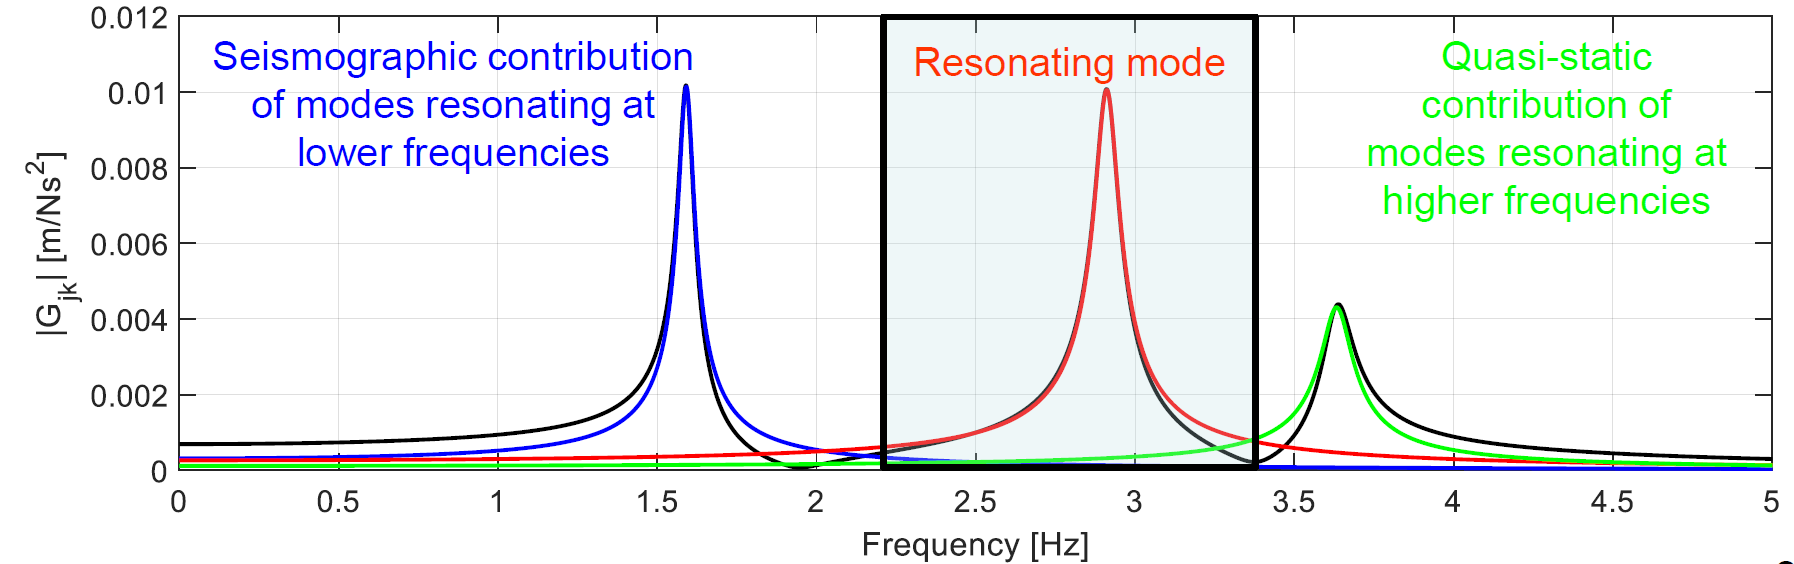
\includegraphics[scale=0.4]{frf_num_regions}
\end{figure}

The frequency ranges of interest are partitions of the frequency axis. Given the $ N $ well distinguished peaks, we will have $ N $ ranges of interest. We chose to compute the bounds of these ranges as the local minima between one peak and the following one. The following depicts the minima and maxima we considered.

\begin{figure}[h]
	\hspace{-70pt}
	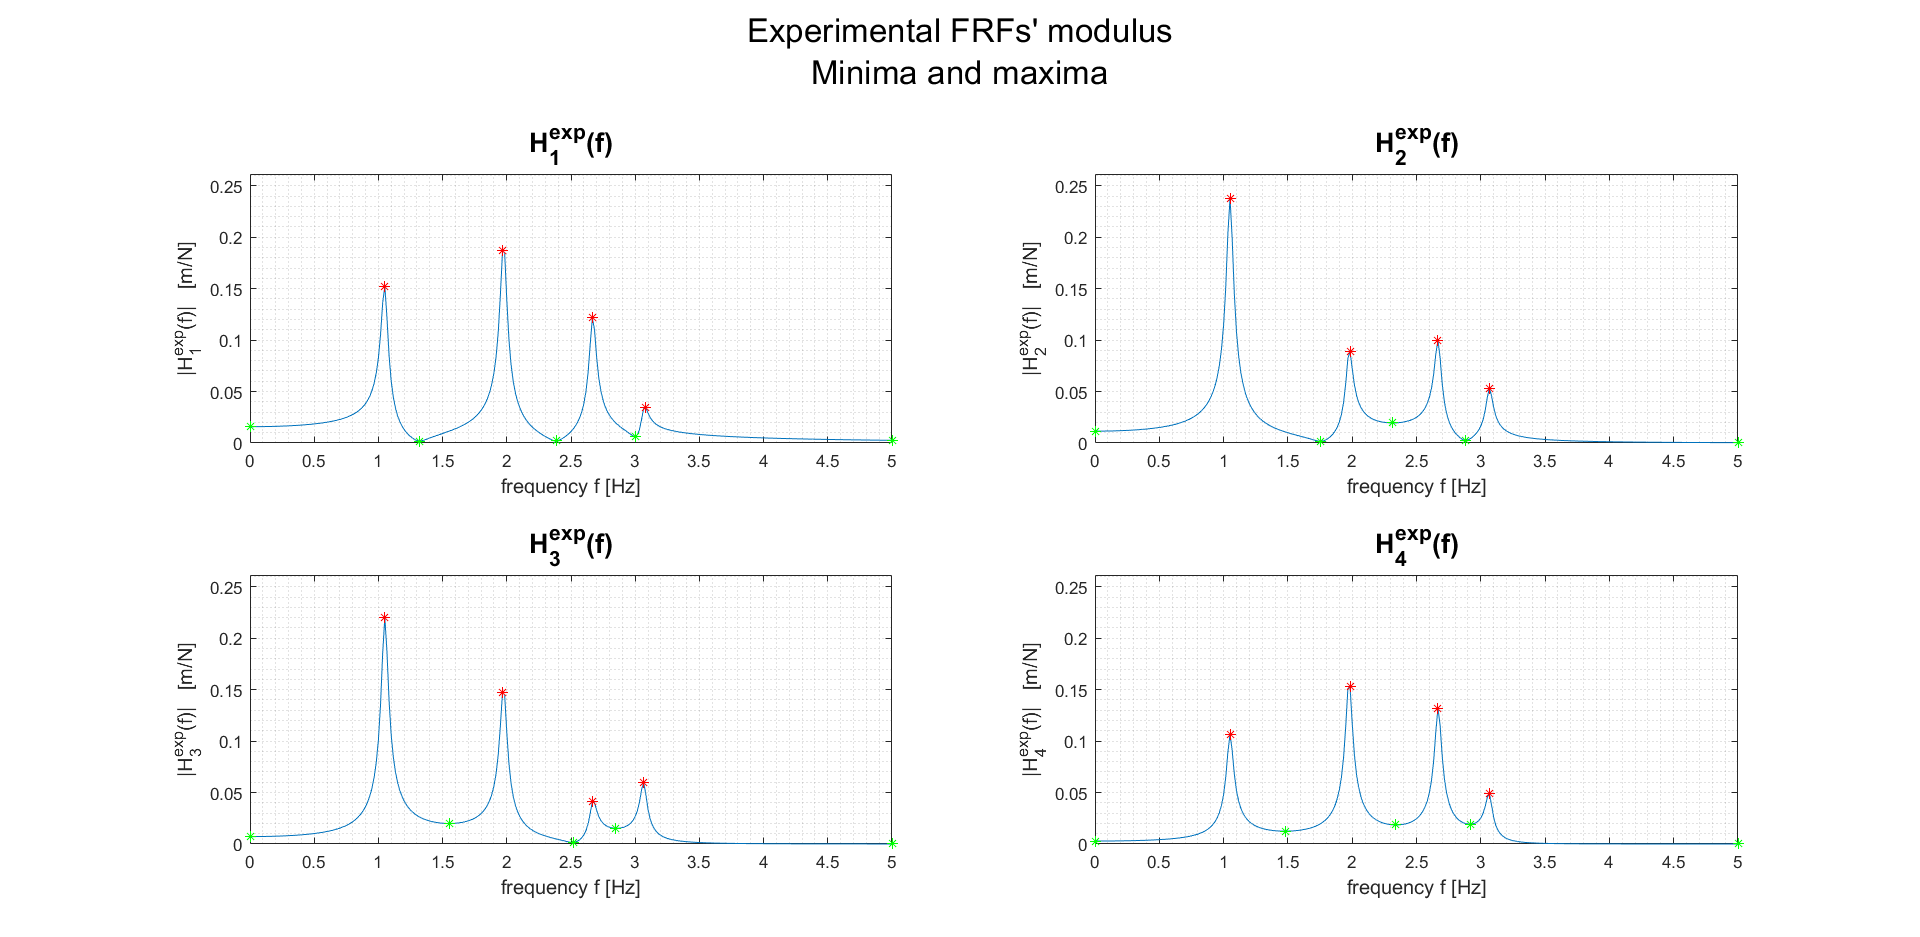
\includegraphics[scale=0.4]{experimental_frfs_modulus_min_max}
\end{figure}

\subsection{Vibration modes identification procedure}

For a given set of experimental FRFs $ H^\textup{exp}_k(\omega) $, obtained for a fixed excitation location and different measurement locations $ k $ (4 points), a least squares minimization procedure can be implemented for the estimation of the modal parameters.

The error function to be minimized (cost function) is:

\[
	\varepsilon = \sum_{s=s_\textup{inf}}^{s_\textup{sup}}
		\Re^2\{H^\textup{exp}_k(\omega_s) - H^\textup{num}_k(\omega_s)\} +
		\Im^2\{H^\textup{exp}_k(\omega_s) - H^\textup{num}_k(\omega_s)\}
\]

Since the error function depends non-linearly on the unknown parameters, an iterative
minimization procedure is used. This is implemented in \textsc{Matlab} throught the function \lstinline!fminsearch!. According to the documentation, \lstinline!fminsearch! is a nonlinear programming solver. It searches for the minimum of a problem specified by $ \min\limits_x f(x) $. Its syntax is: \lstinline!x = fminsearch(fun, x0, options)!.

\lstinline!fun! is the function to minimize, specified as a function handle or function name. \lstinline!fun! is a function that accepts a vector or array \lstinline!x! and returns a real scalar \lstinline!f! (the objective function evaluated at \lstinline!x!).

An initial guess vector \lstinline!x0! (\lstinline!xpar0! in our code) is required, consisting of a preliminary estimate of:

\begin{enumerate}
	\item $ \omega_{\textup{d}_k}^{(i)} $ which is found from the maximum peak in the considered frequency range. We already discussed the procedure in section \ref{sec:simplified_methods}. It has been evaluated from each FRF and then averaged.
	\item $ \xi_k^{(i)} $ which is found through a simplified method (in our case the half power bandwidth method). We already discussed the procedure in section \ref{sec:simplified_methods}. It has been evaluated from each FRF and then averaged.
	\item $ A_k^{(i)} $ which is found considering each FRF at resonance and assuming real valued mode shapes (valid in resonance condition):

\[
	\phi^{(i)}_k =
		- \Im\{H^{\textup{exp}}_k(\omega_{\textup{d}_k}^{(i)})\} \,
		\omega_{\textup{d}_k}^{(i)} c^{(i)}_k	= A^{(i)}_k
\]

Again, we already discussed the procedure in section \ref{sec:simplified_methods}.
It follows that $ B^{(i)}_k = 0 $.
	\item $C^{(i)}_k , D^{(i)}_k, E^{(i)}_k, 	F^{(i)}_k $ are set to zero under the assumption of sufficiently distinguished peaks.
\end{enumerate}

The non-linear minimization procedure elaborates separately the FRFs, leading to an estimate of the modal parameters $ \omega_{\textup{d}_k}^{(i)}, \xi_k^{(i)}, A_k^{(i)} $ for every frequency range (i.e. for every peak) and for every measurement. Then the parameters are averaged. 
A further improvement of the algorithm could be to perform the minimization simultaneously on the whole set of FRFs, leading to a more precise estimate of the modal parameters. In this case the information given by the correlation of the FRFs is exploited. The quality of the estimates can be visually assessed comparing in a plot the identified FRFs $ H^\textup{num}_k(\omega) $ with the experimental ones $ H^\textup{exp}_k(\omega) $: we may conclude the algorithm already worked very well in general. The major flow is in the last phase plot: a $ +90^\circ $ jump is shown, as if an anti-resonance were present after the FRF's pole.

\begin{figure}[h]
	\hspace{-70pt}
	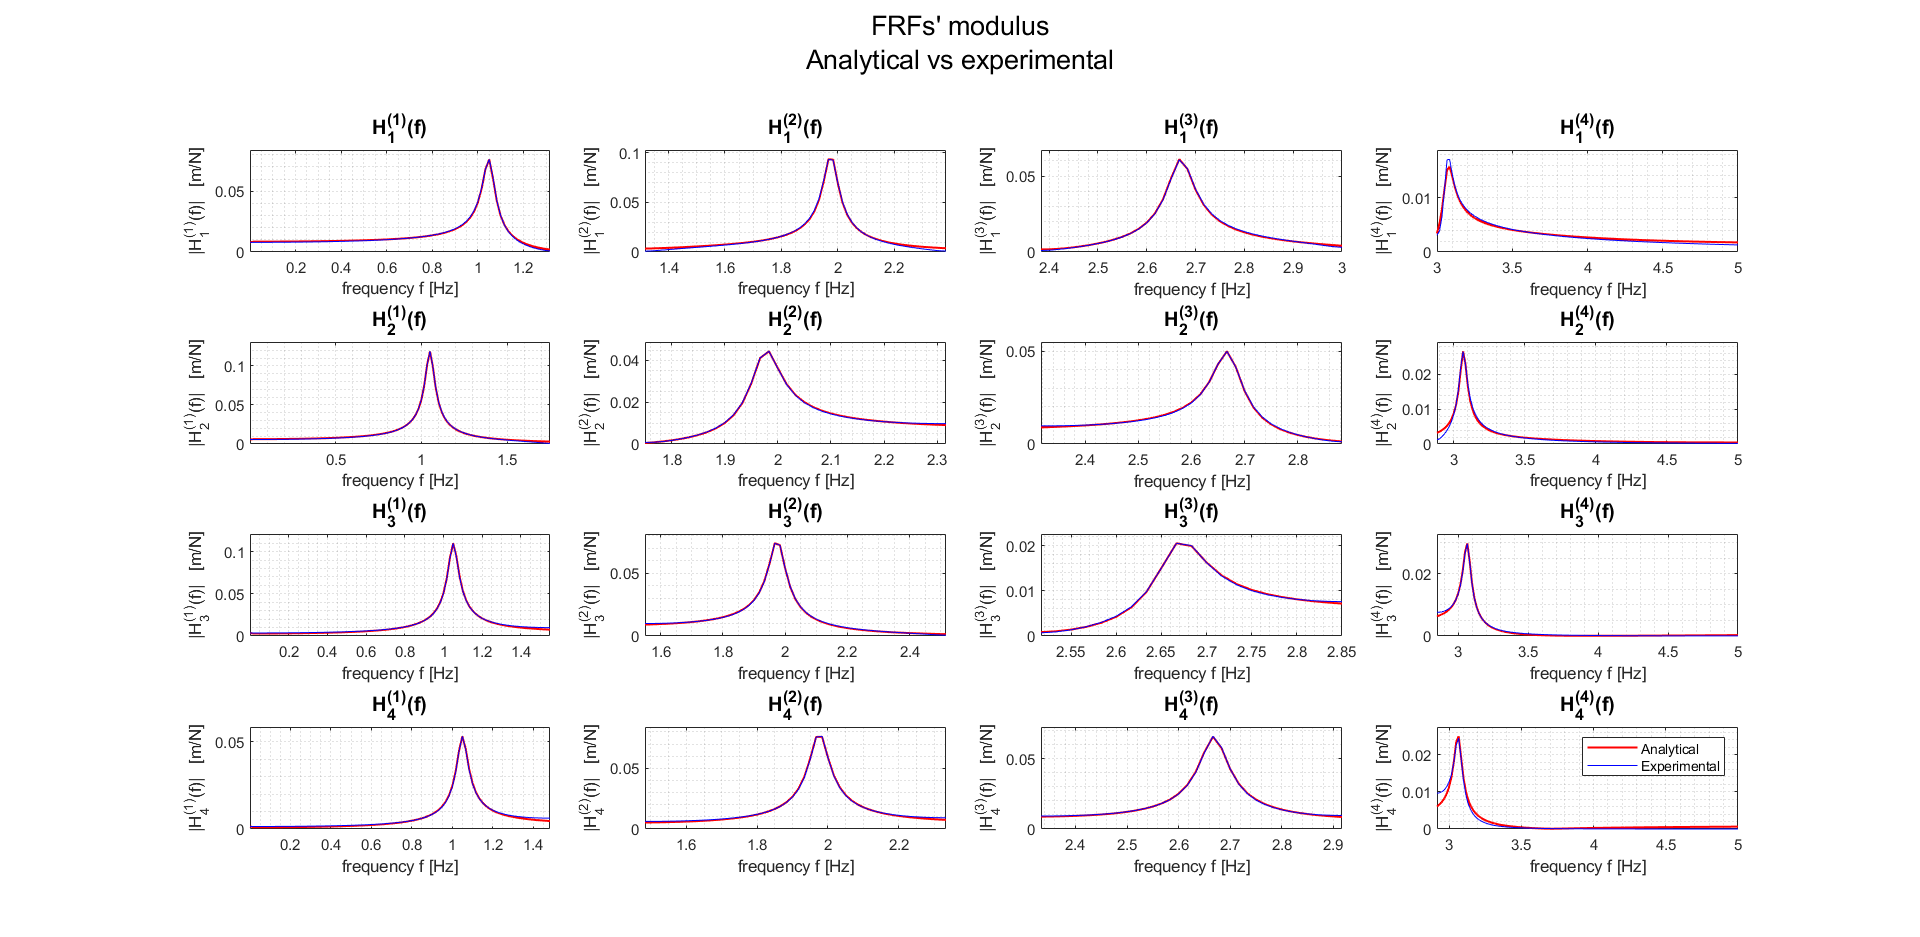
\includegraphics[scale=0.4]{frfs_anal_vs_exp_modulus}
\end{figure}

\begin{figure}[H]
	\hspace{-70pt}
	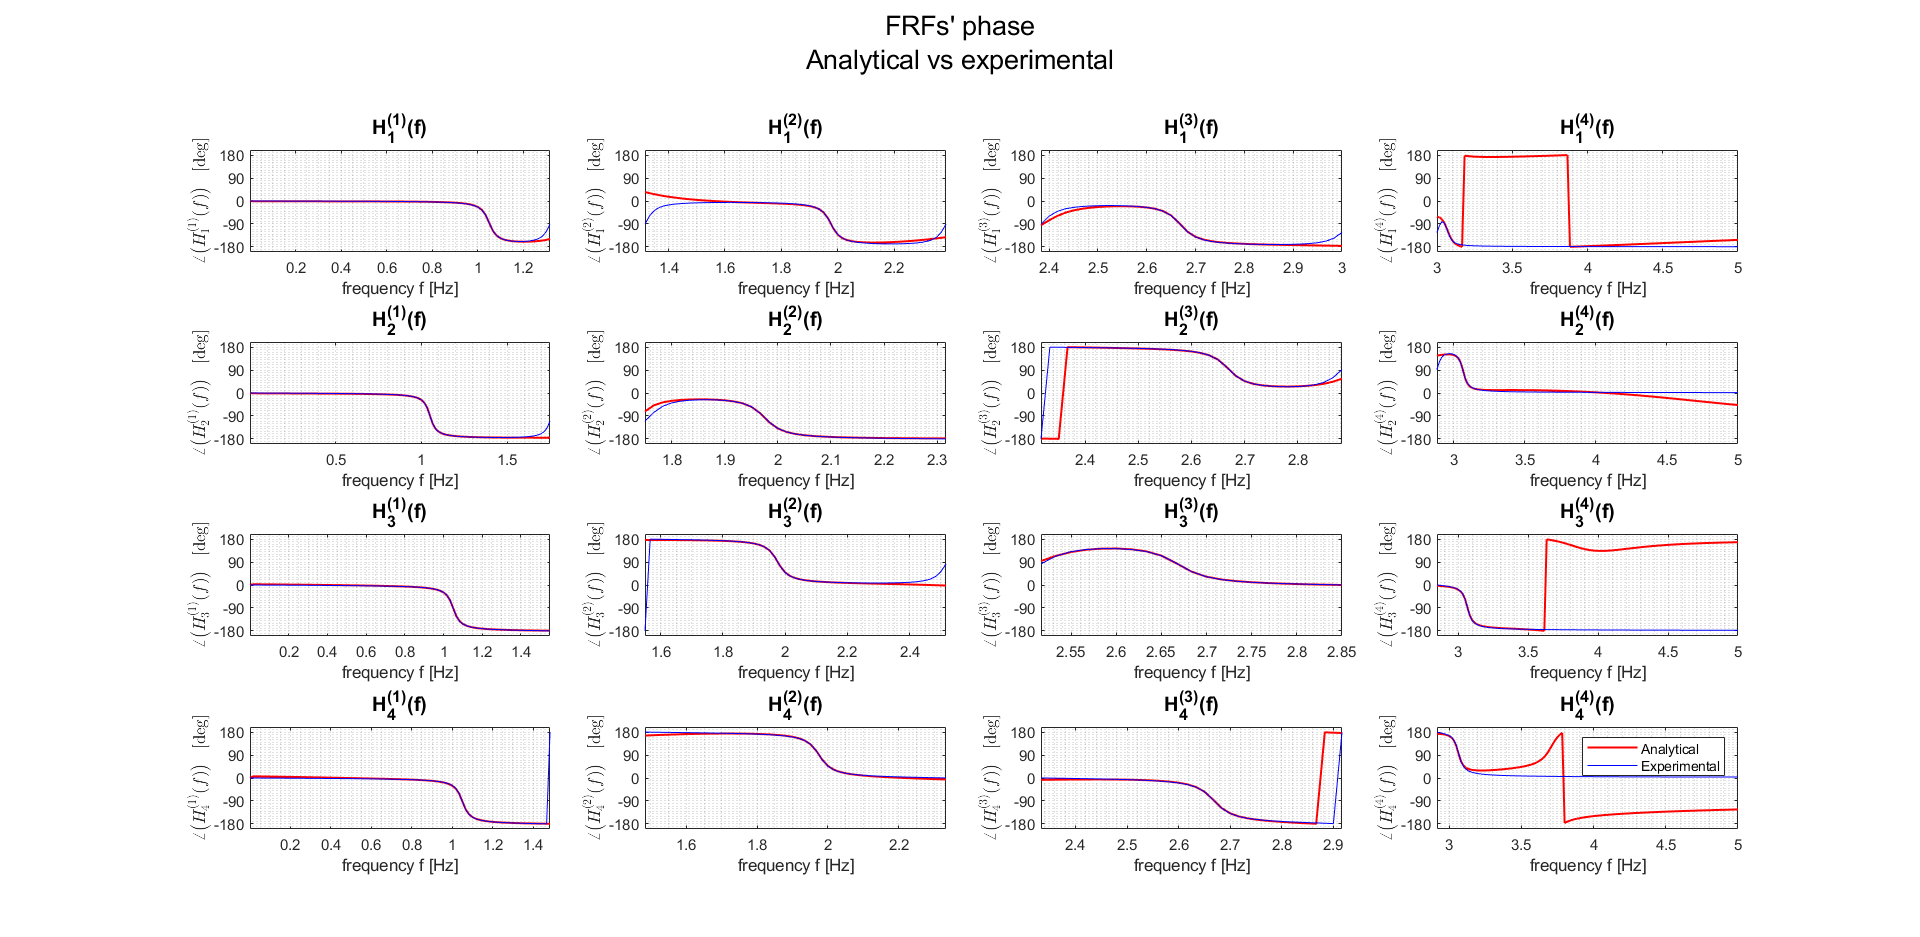
\includegraphics[scale=0.4]{frfs_anal_vs_exp_phase}
\end{figure}


\section{Modal parameter comparison}

The estimated modal parameters have been reduced to a single value per mode as for the simplified methods of section \ref{sec:simplified_methods}, averaging among the measurements and resulting in the following vectors:

\[
	\mathbf{f_d} =	\begin{bmatrix}
										1.050 & 1.975 & 2.669 & 3.068
									\end{bmatrix} \text{~ , ~}
		\bm{\xi} =	\begin{bmatrix}
									0.0159 & 0.0136 & 0.0100 & 0.0092
								\end{bmatrix}
\]

Instead, the normalized modal matrix is

\[
	\bm{\phi} =	\begin{bmatrix}
								1				& 1				& 1				& 1 \\
								1.5632	& 0.4579	& -0.8252	& -1.4745 \\
								1.4459	& -0.8050 & -0.3504	& 1.7016 \\
								0.7000	& -0.8510 & 1.1423	& -1.5256 \\
							\end{bmatrix}
\]

All the results are very similar to those obtained with the simplified approach. The greatest divergences are found in the modal matrix, which now should be more accurate.


\section{FRFs reconstruction}

Employing a modal approach, we will reconstruct the FRFs and compare them with the original ones.

In our \textsc{Matlab} script the variable \lstinline!vpar! contains all the modal parameters found through the minimization process, for each measurement and for each mode. Putting those modal parameters in the equation \eqref{eqn:h_exp_modal}, implemented in the function \lstinline!reco!, we were able to reconstruct the FRFs. 

\begin{figure}[H]
	\hspace{-70pt}
	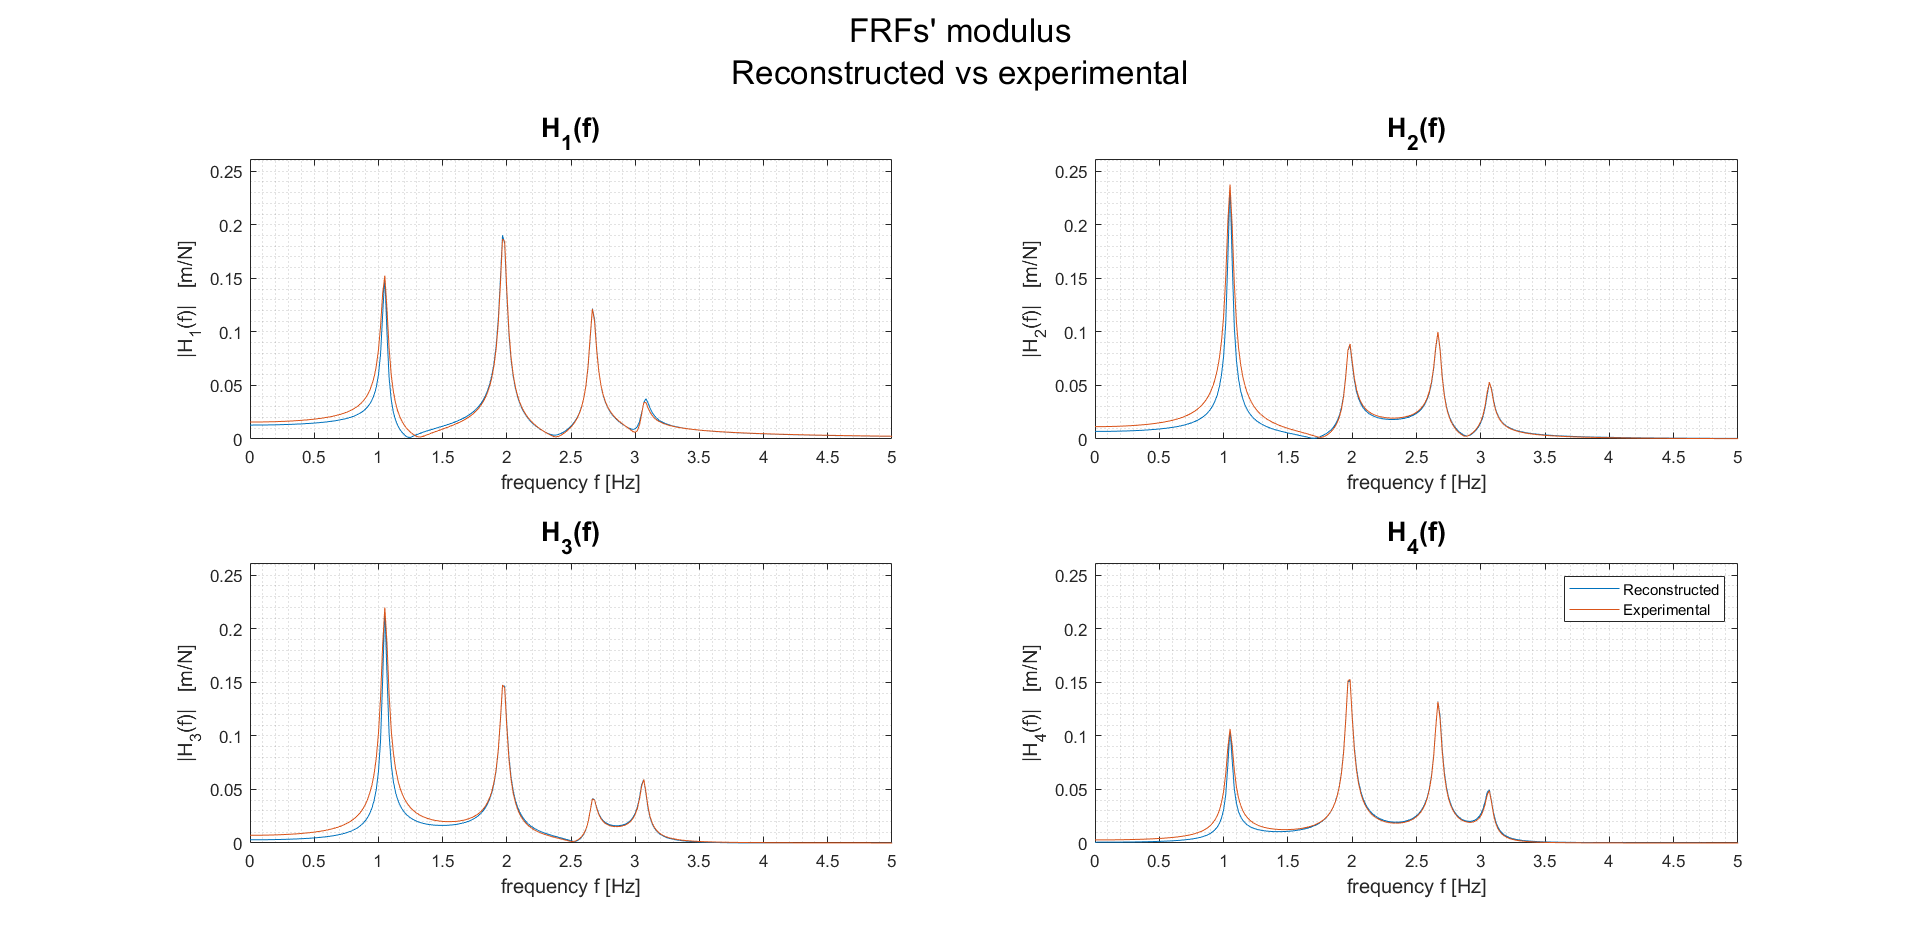
\includegraphics[scale=0.4]{frfs_rec_vs_exp_modulus}
\end{figure}

\begin{figure}[H]
	\hspace{-70pt}
	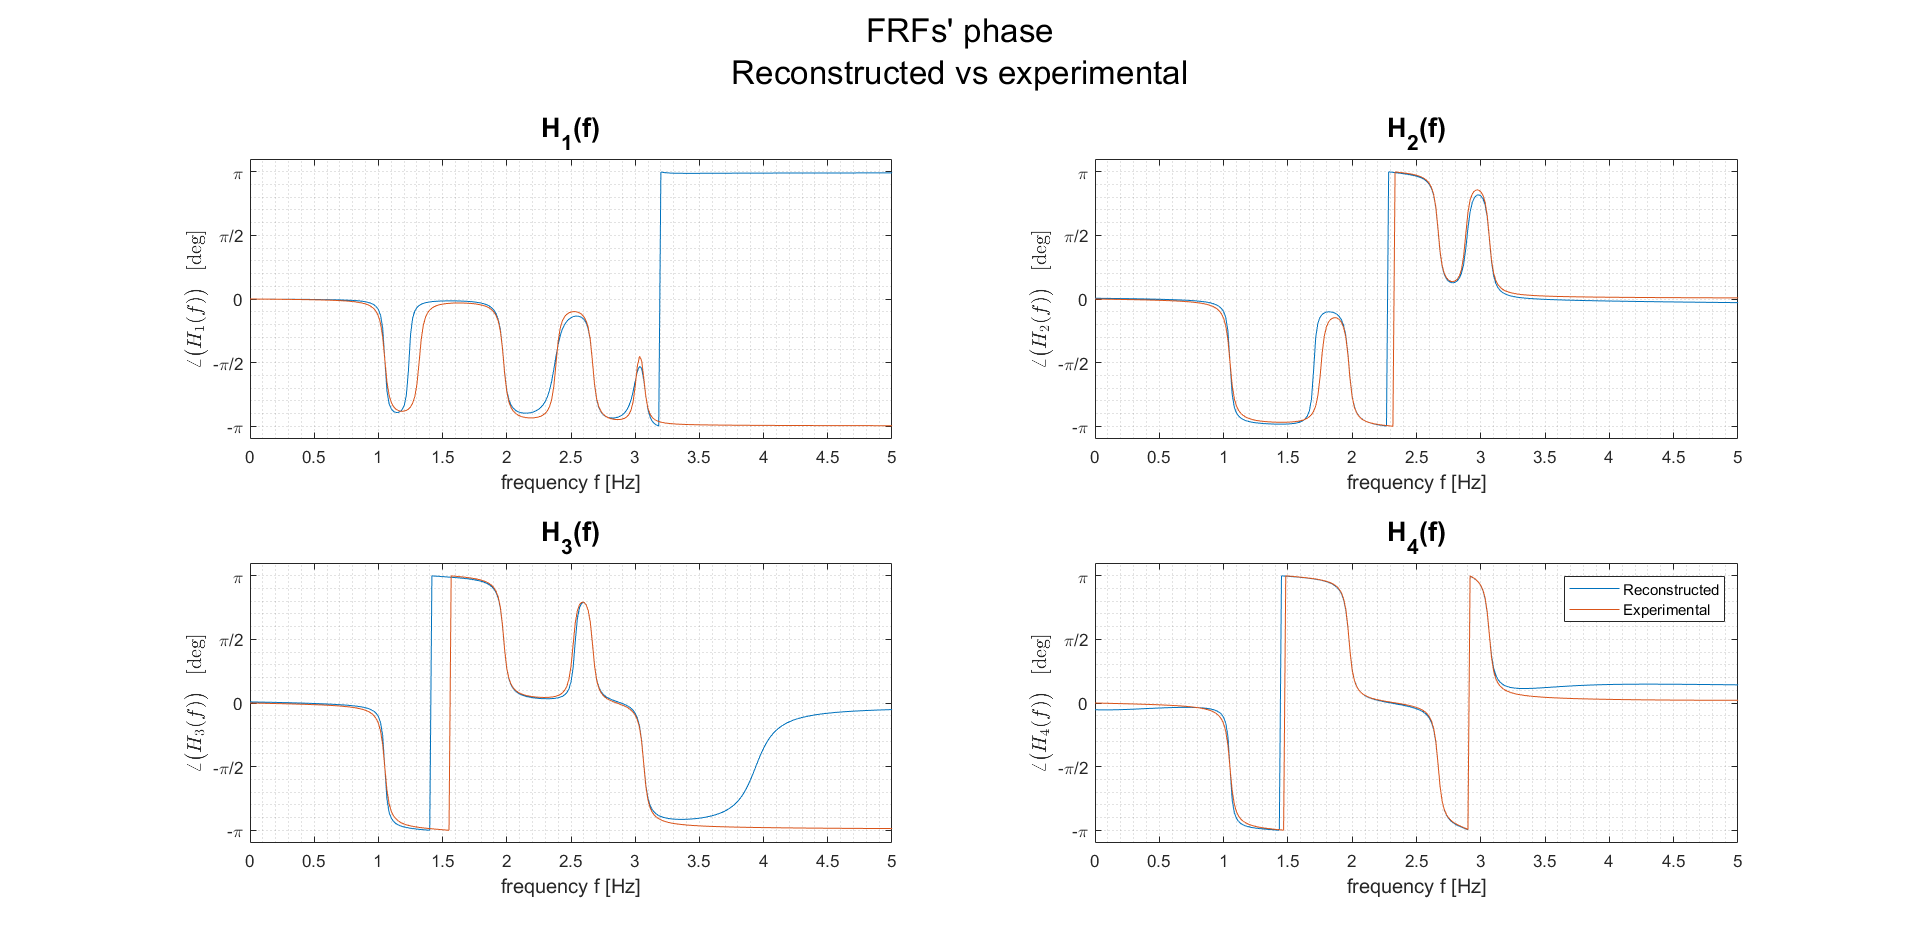
\includegraphics[scale=0.4]{frfs_rec_vs_exp_phase}
\end{figure}

The previous plots represent respectively amplitude and phase of the reconstructed FRFs in comparison with the experimental ones.
It can be seen that the reconstruction is very much close both in amplitude and in phase, as we could predict from the previous plots.


\part*{EXTRA}

\section{Co-located FRF for $ x_2 $}

The requested co-located FRF is the second element on the diagonal of the Frequency Response Matrix of the system. To reconstruct this matrix, we chose to first reconstruct the modal FRM, computing the modal FRFs thanks to the modal mass, damping and stiffness matrices obtained in the minimization process, and then to pass to the system's FRM with the modal matrix $ \bm{\phi} $. The first step was to obtain the modal matrices $ \mathbf{M_q} $, $ \mathbf{C_q} $ and $ \mathbf{K_q} $ from the values stored in \lstinline!vpar!, by computing the mean measurement-wise and then assigning the results to the elements in the diagonal of the matrices:

\[ \begin{split}
	\mathbf{M_q} =	\begin{bmatrix}
										1	& 0	& 0	& 0 \\
										0	& 1	& 0	& 0 \\
										0	& 0	& 1	& 0 \\
										0	& 0	& 0	& 1
									\end{bmatrix} \text{~ , ~}
		\mathbf{C_q} =	\begin{bmatrix}
											0.3347	& 0				& 0				& 0 \\
											0				& 0.3326	& 0				& 0 \\
											0				& 0				& 0.3339	& 0 \\
											0				& 0				& 0				& 0.3566
										\end{bmatrix} \text{~ , ~} \\[10pt]
	\mathbf{K_q} =	\begin{bmatrix}
										43.5295	& 0					& 0					& 0 \\
										0				& 154.0437	& 0					& 0 \\
										0				& 0					& 281.1869	& 0 \\
										0				& 0					& 0					& 371.2903
									\end{bmatrix}
\end{split} \]

Considering the system having these matrices as system parameters, we computed the modal Frequency Response Matrix as usual

\[
	\mathbf{H_q}(\Omega) = \mathbf{D_q}^{-1}(\Omega) =
		(-\Omega^2 \, \mathbf{M_q} + j \Omega \, \mathbf{C_q} + \mathbf{K_q})^{-1}
\]

where $ \mathbf{D_q}(\Omega) $ is the mechanical impedance matrix of the system. The outcome is the following FRM:

\begin{figure}[H]
	\hspace{-70pt}
	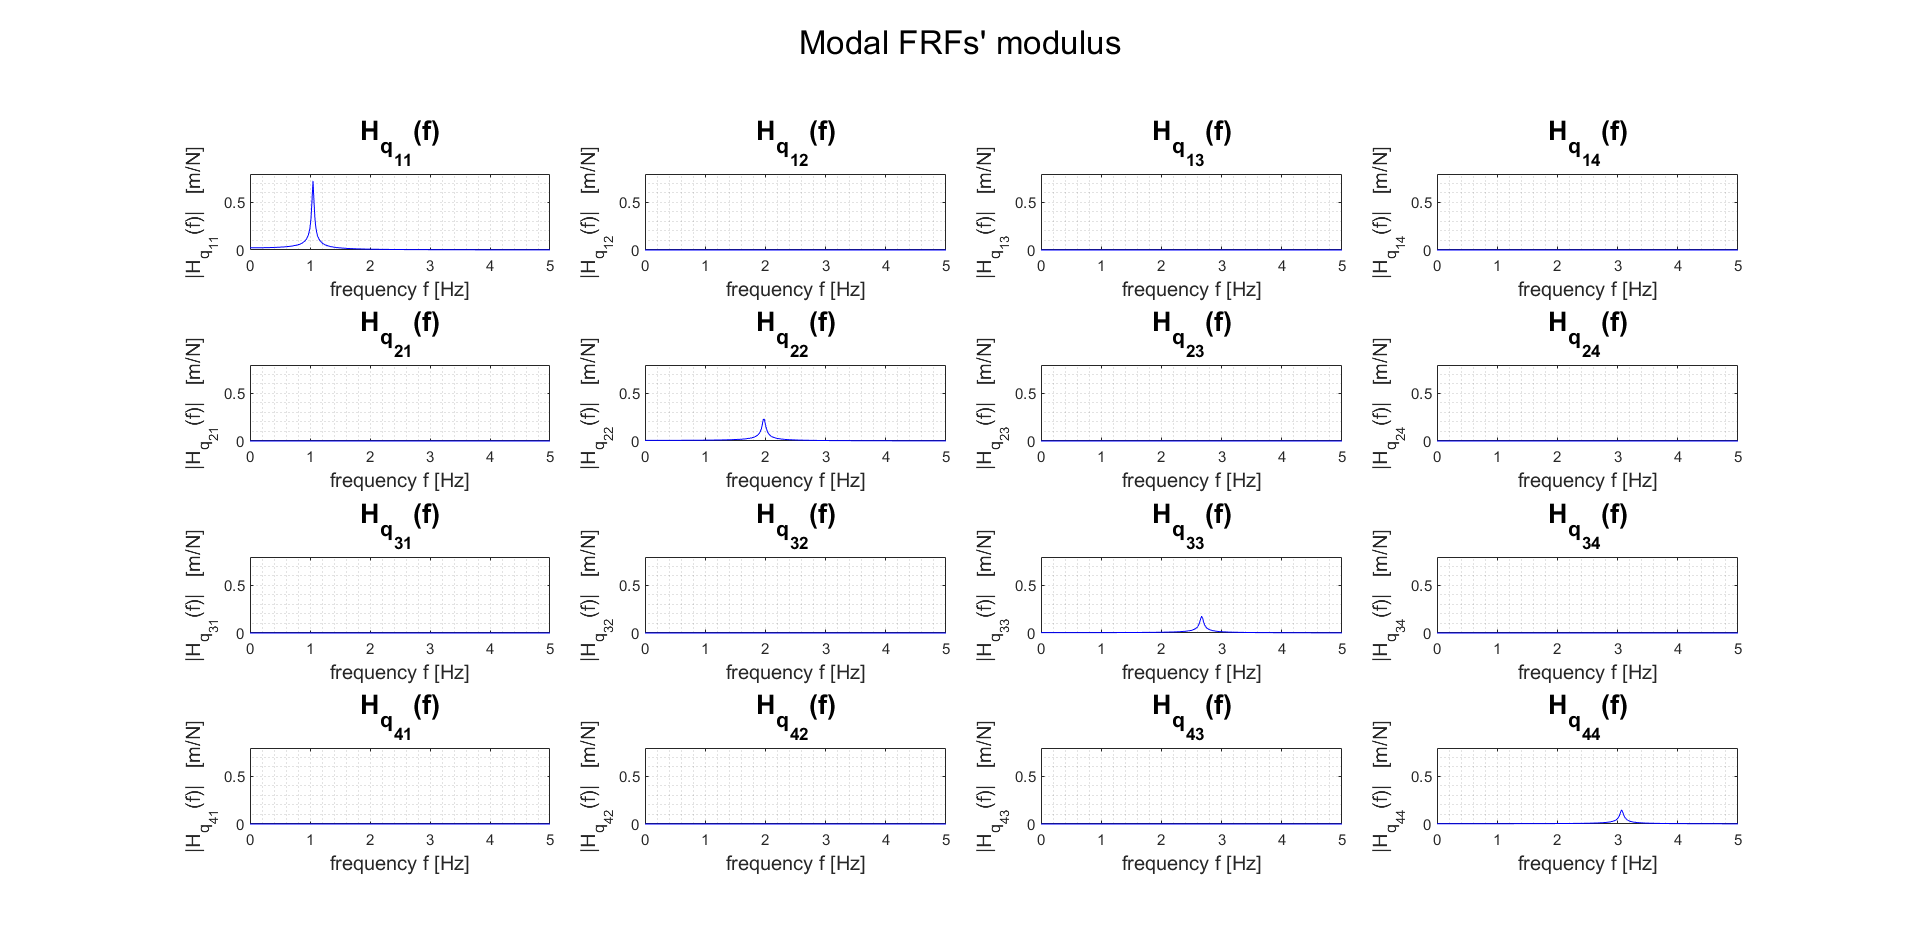
\includegraphics[scale=0.4]{modal_frfs_modulus}
\end{figure}

\begin{figure}[H]
	\hspace{-70pt}
	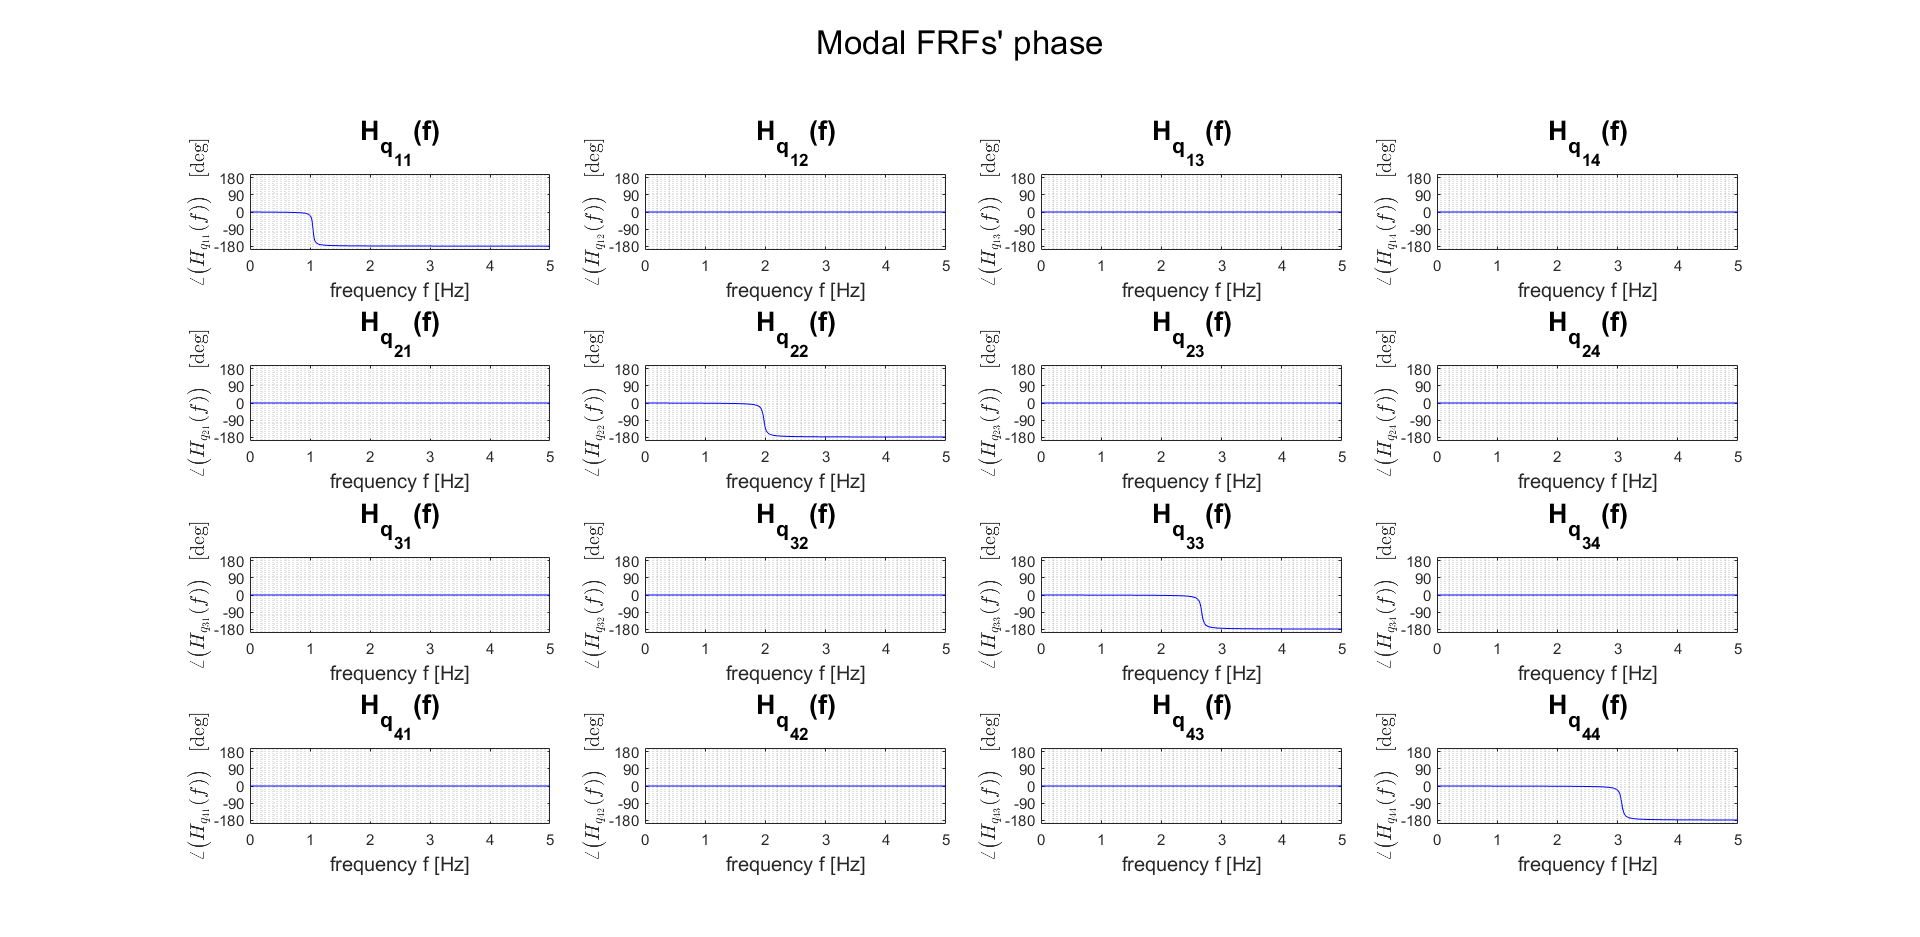
\includegraphics[scale=0.4]{modal_frfs_phase}
\end{figure}

which is diagonal as expected. We then exploited the formula $	\mathbf{H}(\Omega) = \bm{\phi} \, \mathbf{H_q}(\Omega) \, \bm{\phi}^\textup{T} $ to pass from one FRM to the one we need. The system's FRM is depicted in the following plots in terms of magnitude and phase.

\begin{figure}[H]
	\hspace{-70pt}
	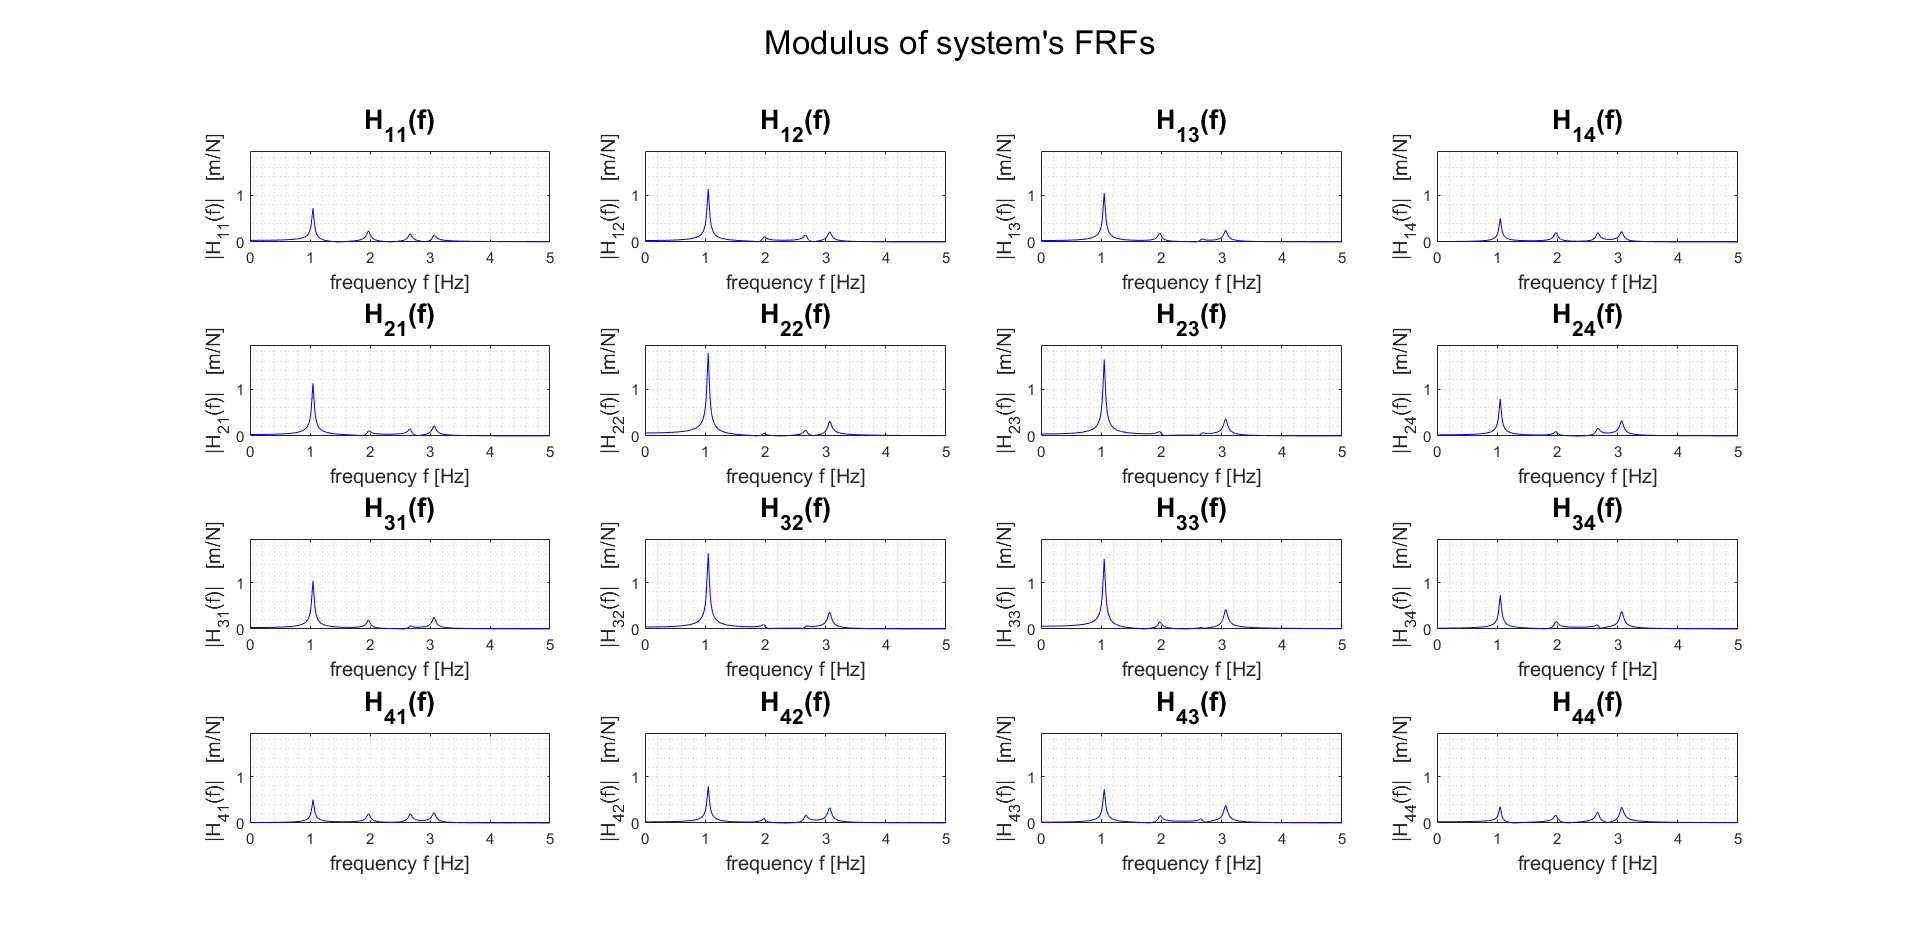
\includegraphics[scale=0.4]{frfs_modulus}
\end{figure}

\begin{figure}[H]
	\hspace{-70pt}
	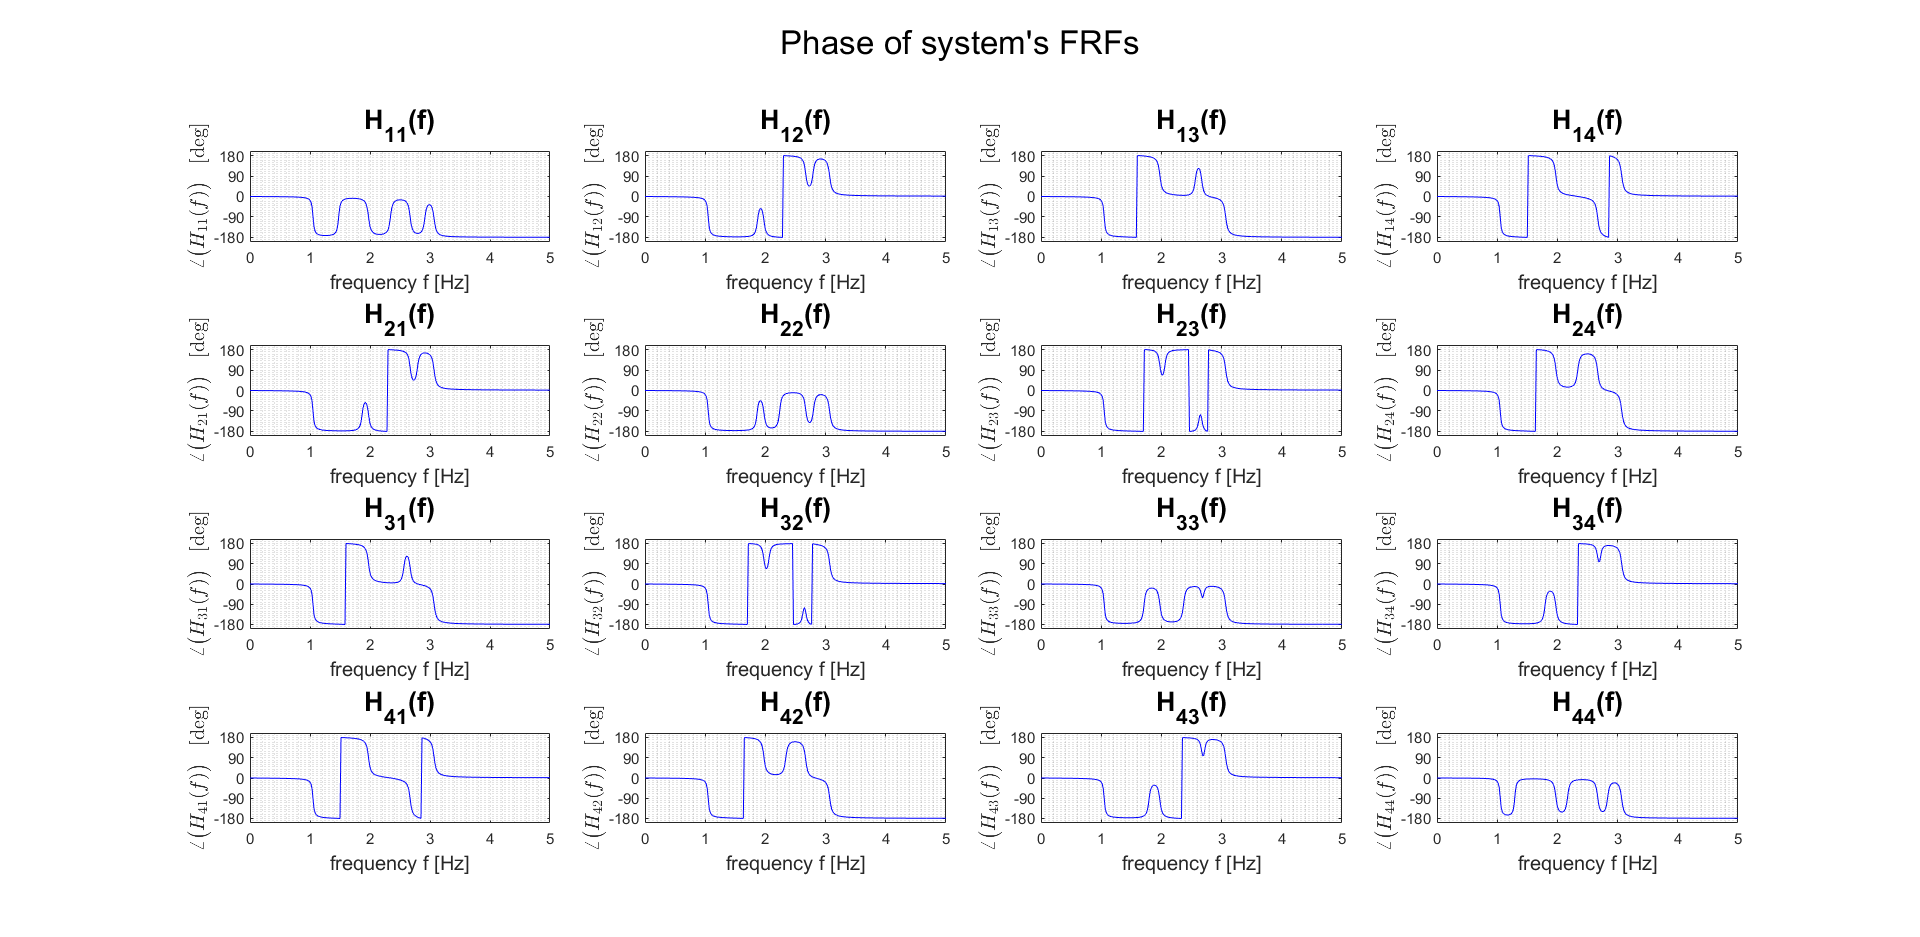
\includegraphics[scale=0.4]{frfs_phase}
\end{figure}

To verify the FRFs are correct, we may compare the first column of the matrix with the four experimental FRFs, which are indeed the transfer functions between the four displacements we were given, seen in this case as independent variables of a 4-degree-of-freedom system, and the force applied to the first one of them. We can see the curves qualitatively coincide, being the difference due to the fact so far we've normalized each mass to $ 1 $. With the correct values of the masses, each peak would be scaled to a different extent so that the FRFs would superimpose with the experimental ones.

\begin{figure}[H]
	\hspace{-70pt}
	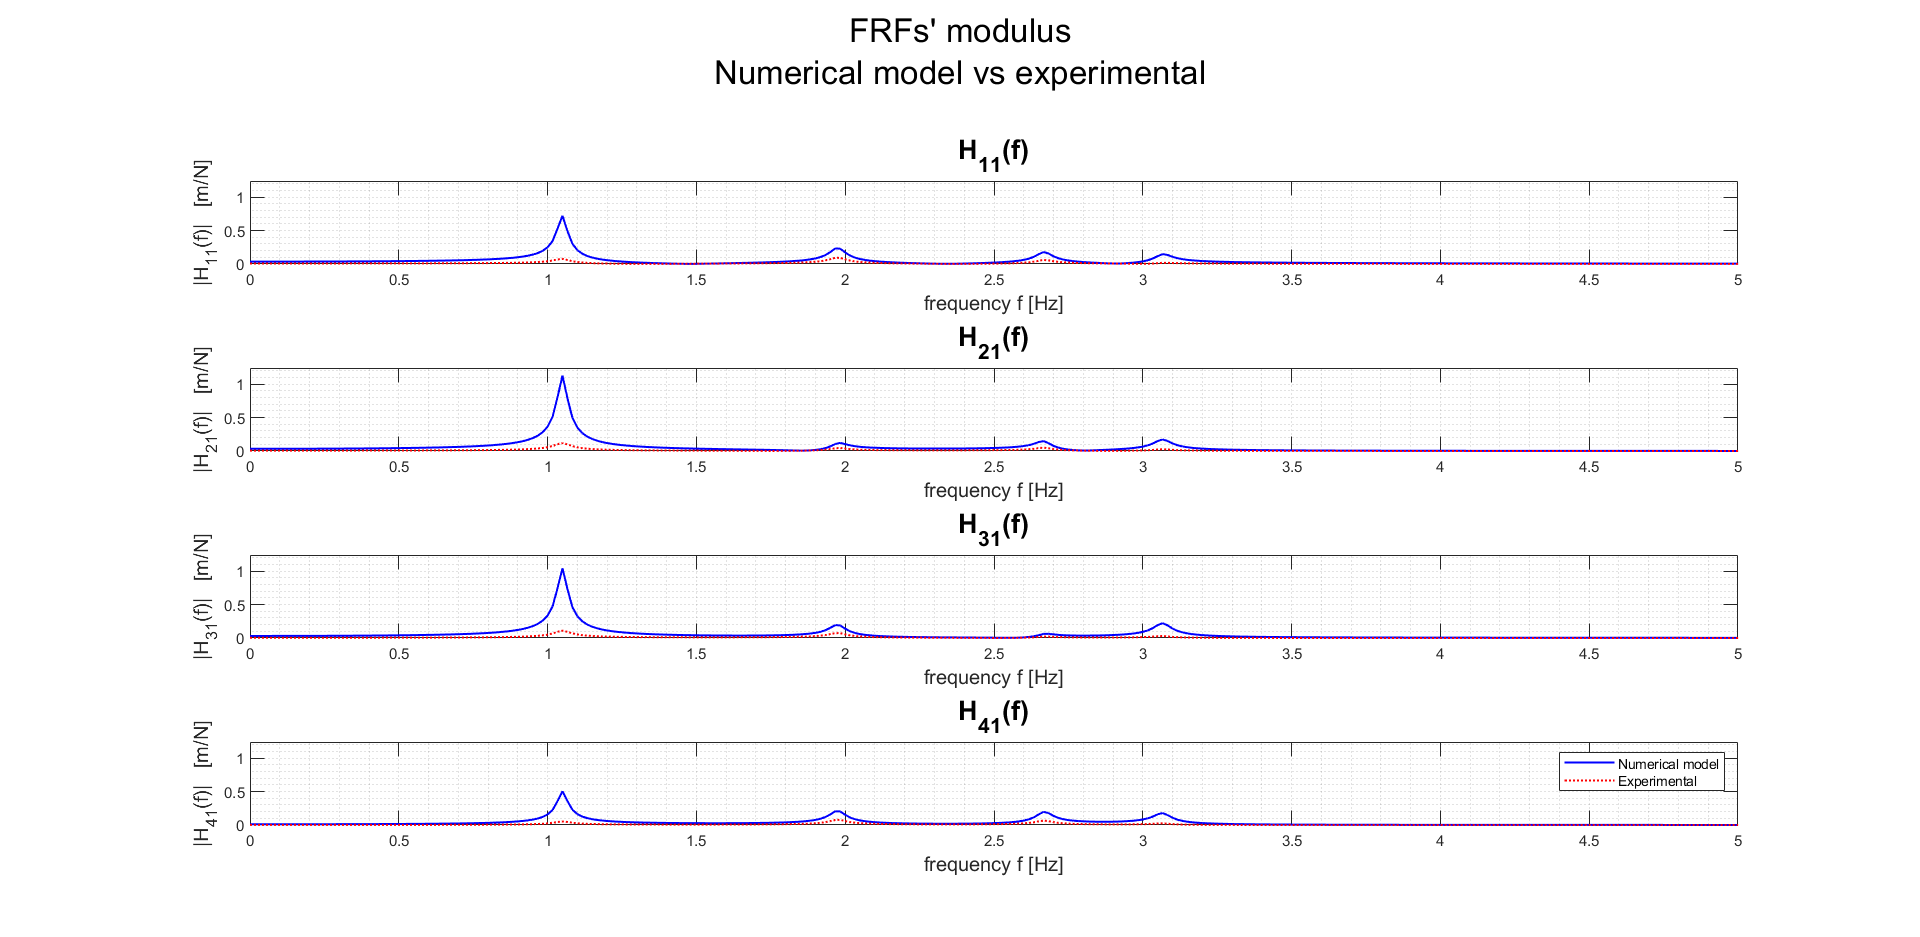
\includegraphics[scale=0.4]{frfs_num_vs_exp_modulus}
\end{figure}

\begin{figure}[H]
	\hspace{-70pt}
	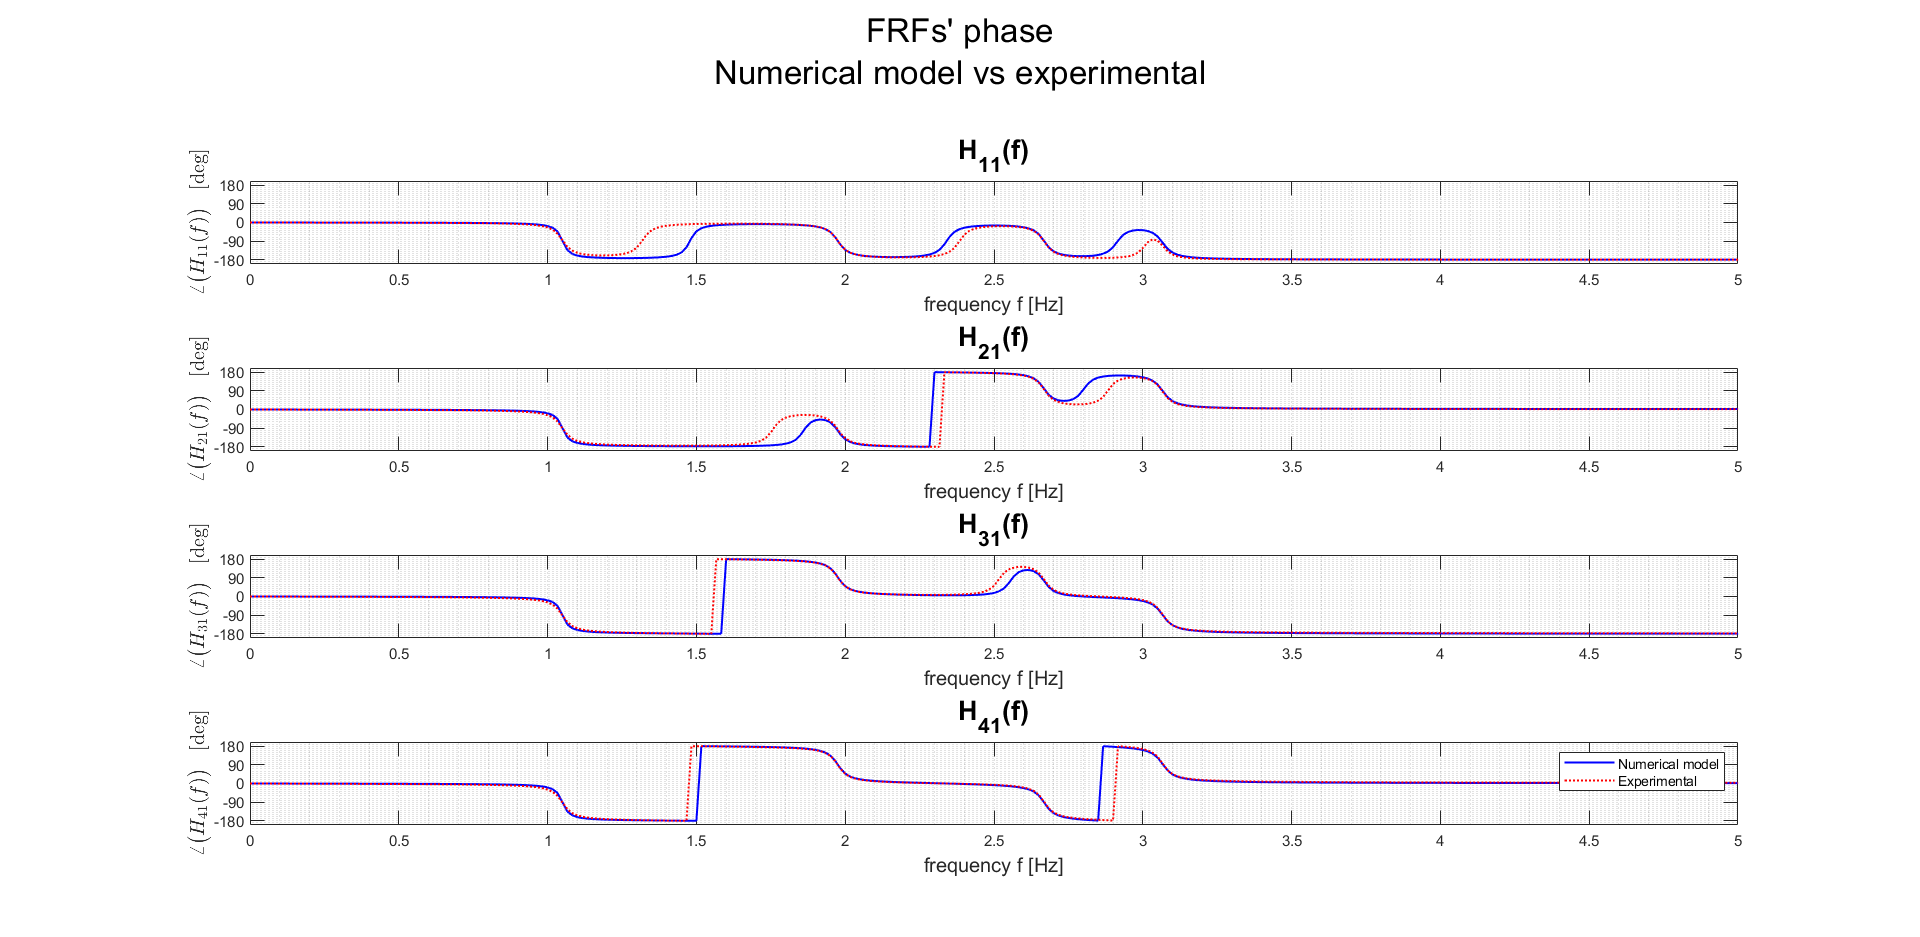
\includegraphics[scale=0.4]{frfs_num_vs_exp_phase}
\end{figure}

The second element on the diagonal is the co-located Frequency Response Function relative to point 2:

\begin{figure}[H]
	\hspace{-70pt}
	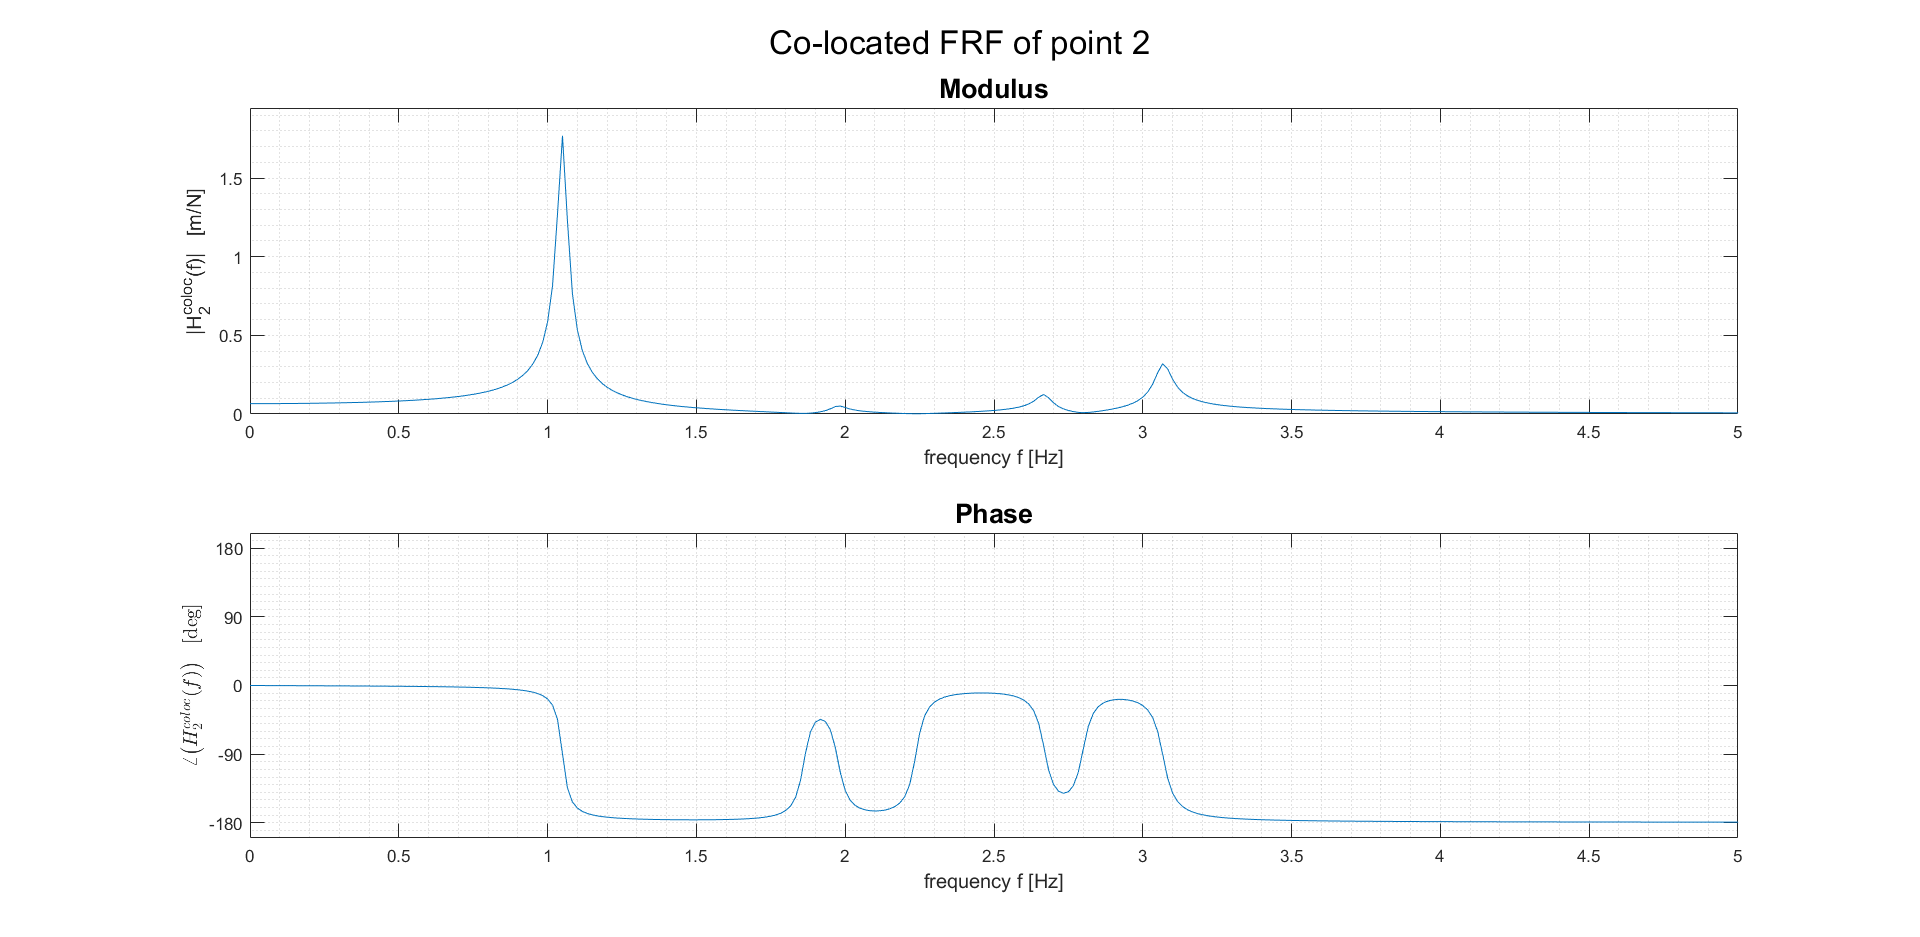
\includegraphics[scale=0.4]{co-located_point2}
\end{figure}


\section{Generalized matrices of numerical model}

Finally, to retrieve the system's matrices, considering the numerical model of the 4-degree-of-freedom system as before, we can proceed using the inverse of the well-known formula (applied only to the mass matrix for the sake of demonstration)

\[
	\mathbf{M_q} = \bm{\phi}^\textup{T} \, \mathbf{M} \, \bm{\phi}
\]

Since $ \bm{\phi} \, \bm{\phi}^\textup{T} \neq \alpha \, \mathbf{I} $, our modes are not orthogonal in strict sense. Therefore, we need to use actual inverse matrix to invert the previous formula. The resulting generalized mass, damping and stiffness matrices are reported here.

\[ \begin{split}
	\mathbf{M} =	\begin{bmatrix}
										0.2984	& 0.0037	& CAZZOOO VIENE NEGATIVO	& 0 \\
										0	& 1	& 0	& 0 \\
										0	& 0	& 1	& 0 \\
										0	& 0	& 0	& 1
									\end{bmatrix} \text{~ , ~}
		\mathbf{C} =	\begin{bmatrix}
											0.3347	& 0				& 0				& 0 \\
											0				& 0.3326	& 0				& 0 \\
											0				& 0				& 0.3339	& 0 \\
											0				& 0				& 0				& 0.3566
										\end{bmatrix} \text{~ , ~} \\[10pt]
	\mathbf{K} =	\begin{bmatrix}
										43.5295	& 0					& 0					& 0 \\
										0				& 154.0437	& 0					& 0 \\
										0				& 0					& 281.1869	& 0 \\
										0				& 0					& 0					& 371.2903
									\end{bmatrix}
\end{split} \]


\end{document}